% Options for packages loaded elsewhere
\PassOptionsToPackage{unicode}{hyperref}
\PassOptionsToPackage{hyphens}{url}
%
\documentclass[
  a4paper]{article}
\usepackage{lmodern}
\usepackage{amssymb,amsmath}
\usepackage{ifxetex,ifluatex}
\ifnum 0\ifxetex 1\fi\ifluatex 1\fi=0 % if pdftex
  \usepackage[T1]{fontenc}
  \usepackage[utf8]{inputenc}
  \usepackage{textcomp} % provide euro and other symbols
\else % if luatex or xetex
  \usepackage{unicode-math}
  \defaultfontfeatures{Scale=MatchLowercase}
  \defaultfontfeatures[\rmfamily]{Ligatures=TeX,Scale=1}
  \setsansfont[]{Calibri Light}
\fi
% Use upquote if available, for straight quotes in verbatim environments
\IfFileExists{upquote.sty}{\usepackage{upquote}}{}
\IfFileExists{microtype.sty}{% use microtype if available
  \usepackage[]{microtype}
  \UseMicrotypeSet[protrusion]{basicmath} % disable protrusion for tt fonts
}{}
\makeatletter
\@ifundefined{KOMAClassName}{% if non-KOMA class
  \IfFileExists{parskip.sty}{%
    \usepackage{parskip}
  }{% else
    \setlength{\parindent}{0pt}
    \setlength{\parskip}{6pt plus 2pt minus 1pt}}
}{% if KOMA class
  \KOMAoptions{parskip=half}}
\makeatother
\usepackage{xcolor}
\IfFileExists{xurl.sty}{\usepackage{xurl}}{} % add URL line breaks if available
\IfFileExists{bookmark.sty}{\usepackage{bookmark}}{\usepackage{hyperref}}
\hypersetup{
  hidelinks,
  pdfcreator={LaTeX via pandoc}}
\urlstyle{same} % disable monospaced font for URLs
\usepackage[margin=1in]{geometry}
\usepackage{graphicx,grffile}
\makeatletter
\def\maxwidth{\ifdim\Gin@nat@width>\linewidth\linewidth\else\Gin@nat@width\fi}
\def\maxheight{\ifdim\Gin@nat@height>\textheight\textheight\else\Gin@nat@height\fi}
\makeatother
% Scale images if necessary, so that they will not overflow the page
% margins by default, and it is still possible to overwrite the defaults
% using explicit options in \includegraphics[width, height, ...]{}
\setkeys{Gin}{width=\maxwidth,height=\maxheight,keepaspectratio}
% Set default figure placement to htbp
\makeatletter
\def\fps@figure{htbp}
\makeatother
\setlength{\emergencystretch}{3em} % prevent overfull lines
\providecommand{\tightlist}{%
  \setlength{\itemsep}{0pt}\setlength{\parskip}{0pt}}
\setcounter{secnumdepth}{-\maxdimen} % remove section numbering
\usepackage{fancyhdr}
\usepackage[T1]{fontenc}
\usepackage[default]{sourcesanspro}
\usepackage{tikz}
\addtolength{\headheight}{1.0cm} 
\fancypagestyle{plain}{} 
\thispagestyle{fancy} 
\renewcommand{\headrulewidth}{0pt}

% Package for references with numbers
\bibliographystyle{apsrev4-1}
\usepackage[numbers]{natbib}
\setcitestyle{numbers}
\usepackage[brazil]{babel}
\usepackage{amsmath}
\usepackage{titling}

\usepackage{background}

\backgroundsetup{
position={3,0.55},
scale=1.2,
color=black,
opacity=1,
angle=0,
pages=all,
contents={%
  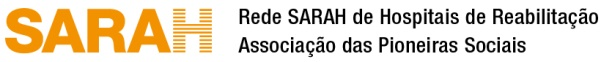
\includegraphics[width=200px,height=200px]{Imagens/logo_header.jpg}
  }%
}
\usepackage{floatrow}
\floatsetup[figure]{capposition=top}
\floatsetup[table]{capposition=top}


\usepackage{fancyhdr}
\pagestyle{fancy}
% center of header
\fancyhf{} % clear all header and footer fields

\renewcommand{\headrulewidth}{0pt}
\usepackage{booktabs}
\usepackage{longtable}
\usepackage{array}
\usepackage{multirow}
\usepackage{wrapfig}
\usepackage{float}
\usepackage{colortbl}
\usepackage{pdflscape}
\usepackage{tabu}
\usepackage{threeparttable}
\usepackage{threeparttablex}
\usepackage[normalem]{ulem}
\usepackage{makecell}
\usepackage{xcolor}

\author{}
\date{\vspace{-2.5em}}

\begin{document}

\rhead{\fontsize{8pt}{10pt} \selectfont Núcleo de Segurança do Paciente
\\ \fontsize{8pt}{10pt} \selectfont Centro Nacional de Controle de Qualidade
}
\begin{center}
 {\LARGE Relatório de Notificações}
\end{center}
\vspace{0.5cm}

\section{NOTIFICAÇÕES – Ano 2021}

\subsection{Quedas Geral}

\begin{table}[H]

\caption{\label{tab:unnamed-chunk-3}Distribuição das quedas mês a mês de acordo com o dano.}
\centering
\resizebox{\linewidth}{!}{
\begin{tabular}[t]{lrrrrrrrrrrrr}
\toprule
 & jan & fev & mar & abr & mai & jun & jul & ago & set & out & nov & Total\\
\midrule
Evento Adverso & 5 & 6 & 9 & 3 & 3 & 1 & 3 & 6 & 1 & 6 & 6 & 49\\
Incidente sem dano & 18 & 19 & 11 & 6 & 10 & 12 & 10 & 15 & 15 & 20 & 17 & 153\\
\midrule
\textbf{Total} & \textbf{23} & \textbf{25} & \textbf{20} & \textbf{9} & \textbf{13} & \textbf{13} & \textbf{13} & \textbf{21} & \textbf{16} & \textbf{26} & \textbf{23} & \textbf{202}\\
\bottomrule
\end{tabular}}
\end{table}

\begin{figure}[H]
\caption{Distribuição da queda de acordo com o período.}
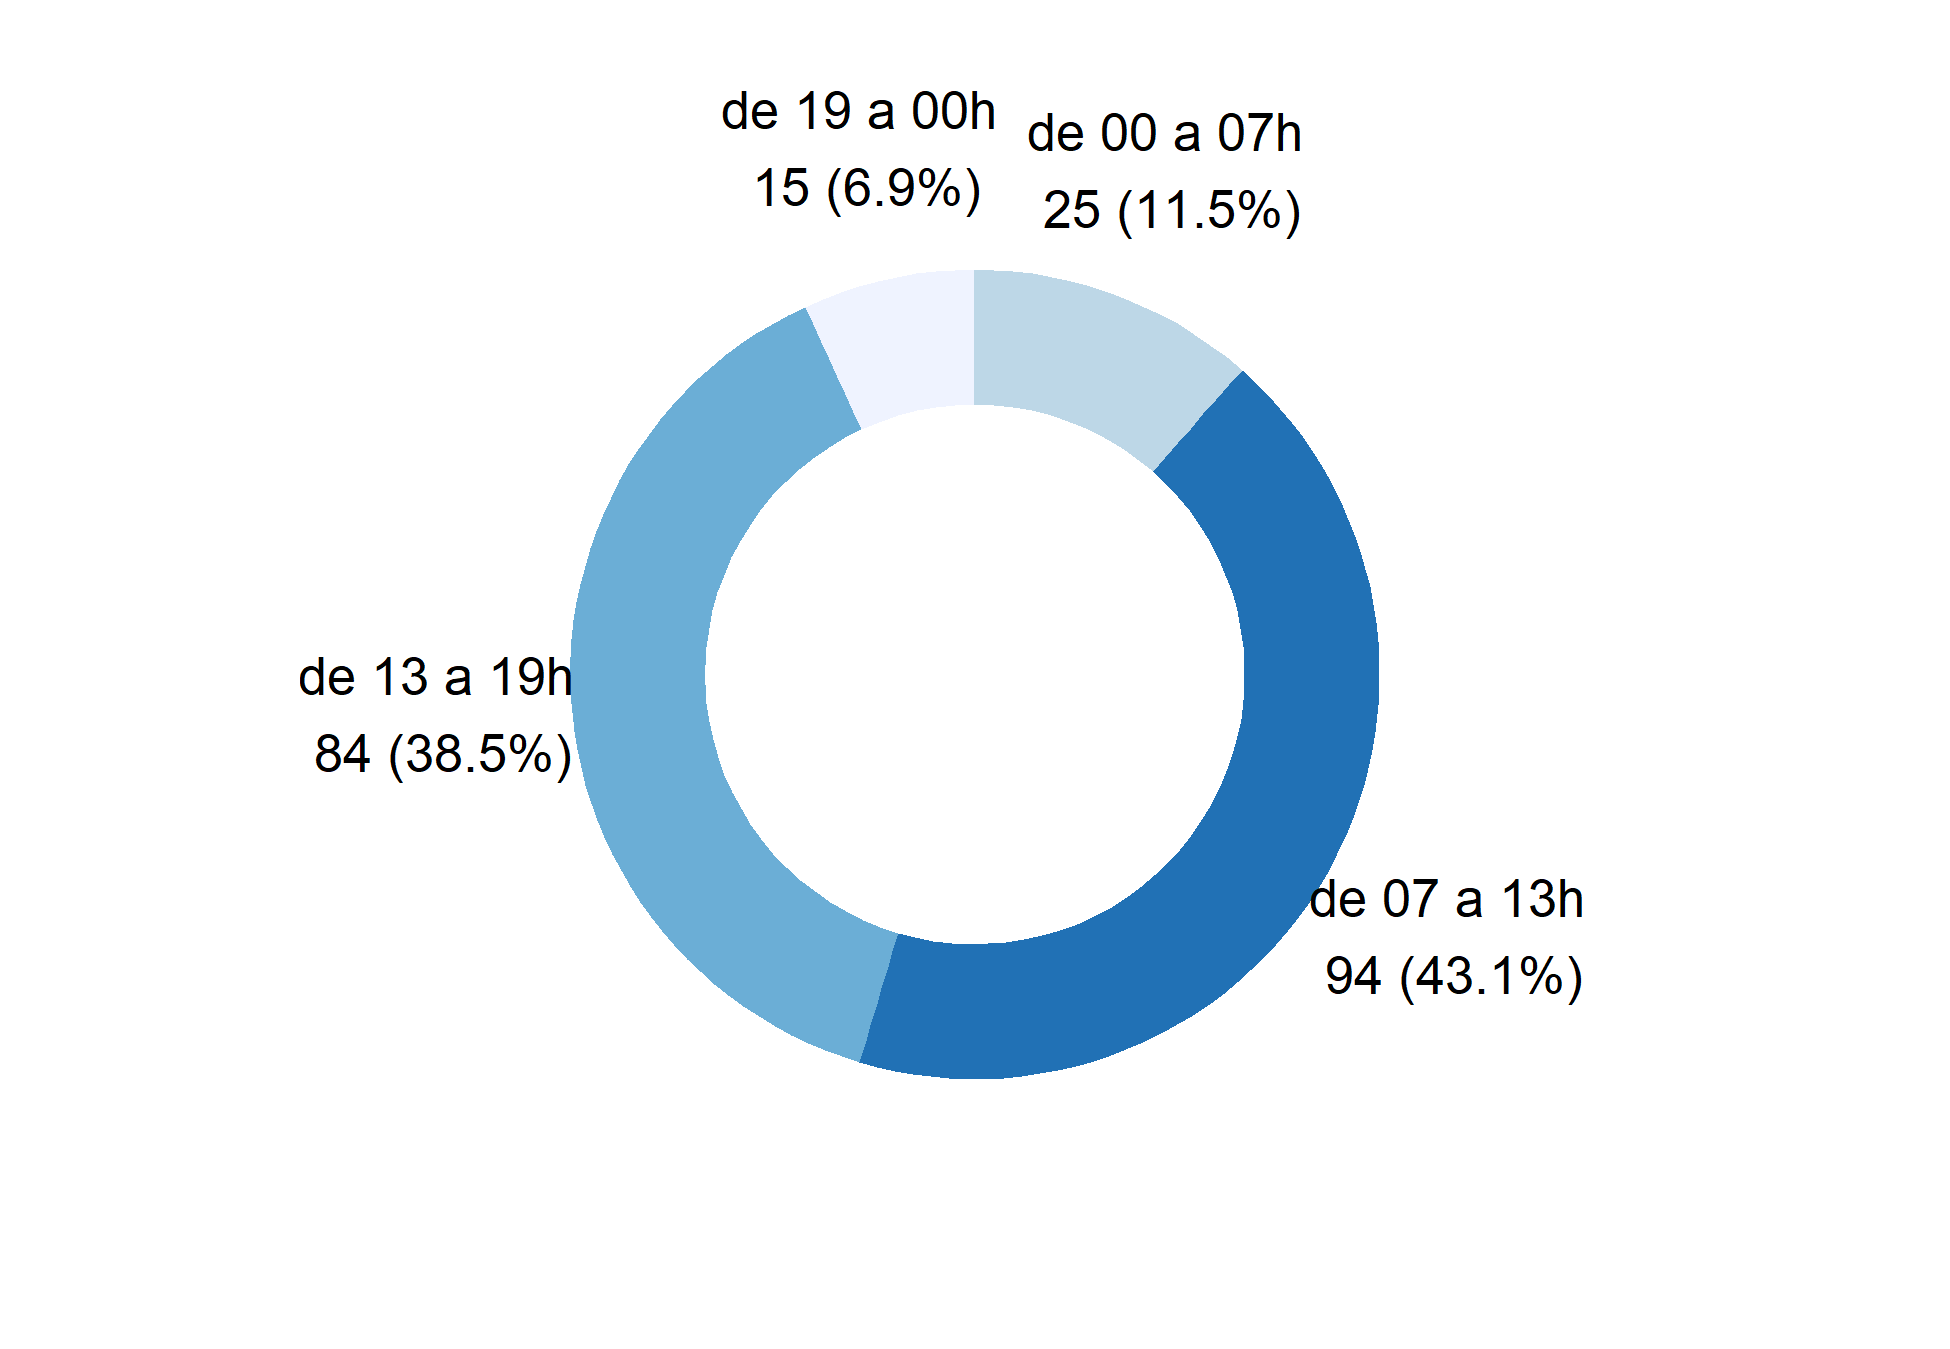
\includegraphics[width=0.7\textwidth]{Imagens/queda_periodo.png}
\end{figure}

\begin{figure}[H]
\caption{Presença de acompanhante no momento da queda.}
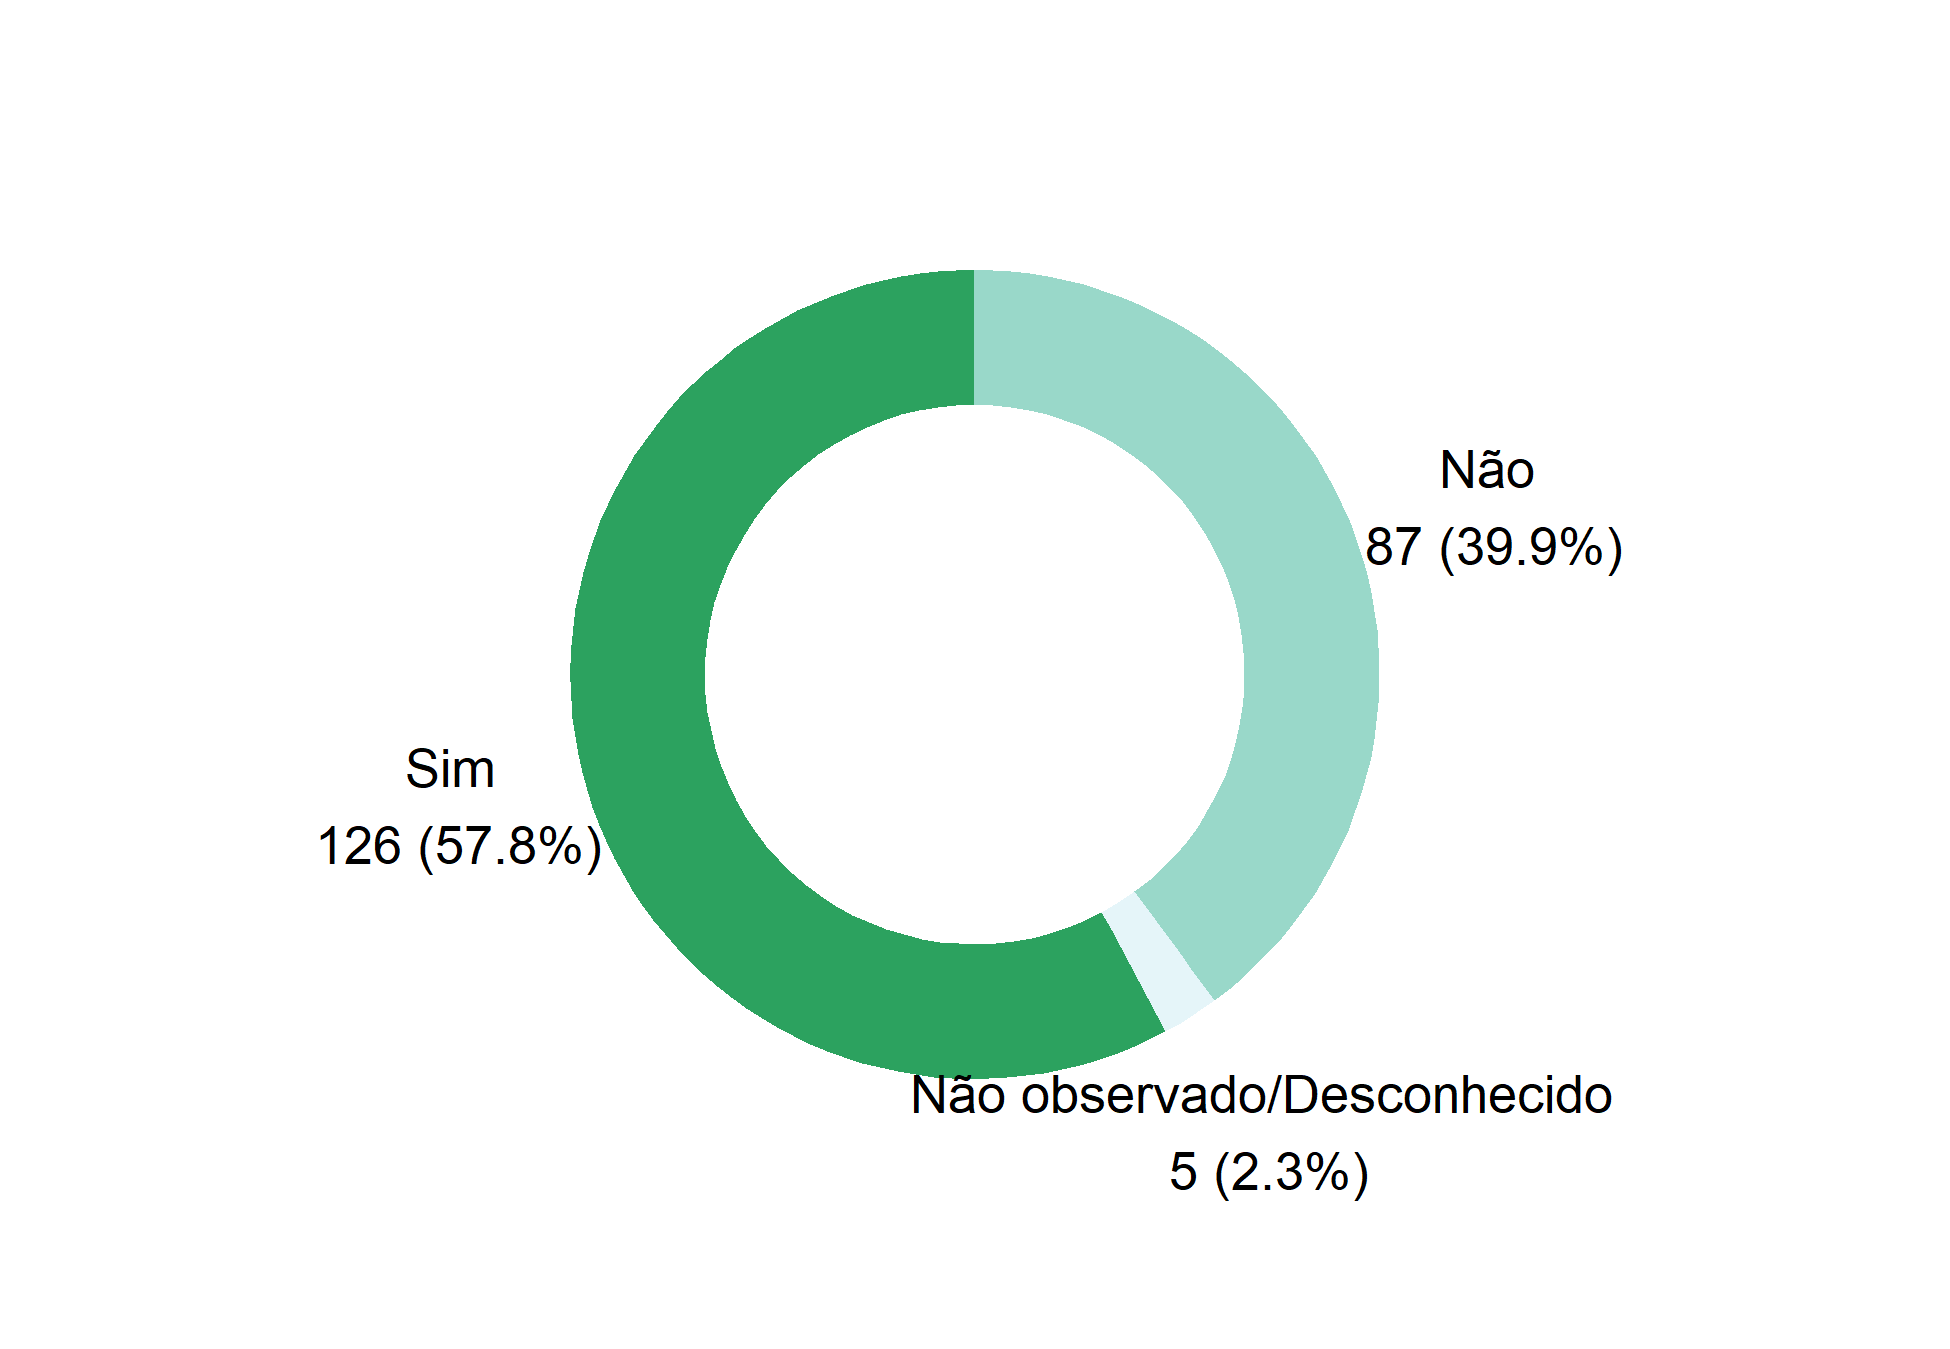
\includegraphics[width=0.7\textwidth]{Imagens/queda_acomp.png}
\end{figure}

\begin{figure}[H]
\caption{Distribuição do gênero nas notificações em Procedimento Cirúrgico.}
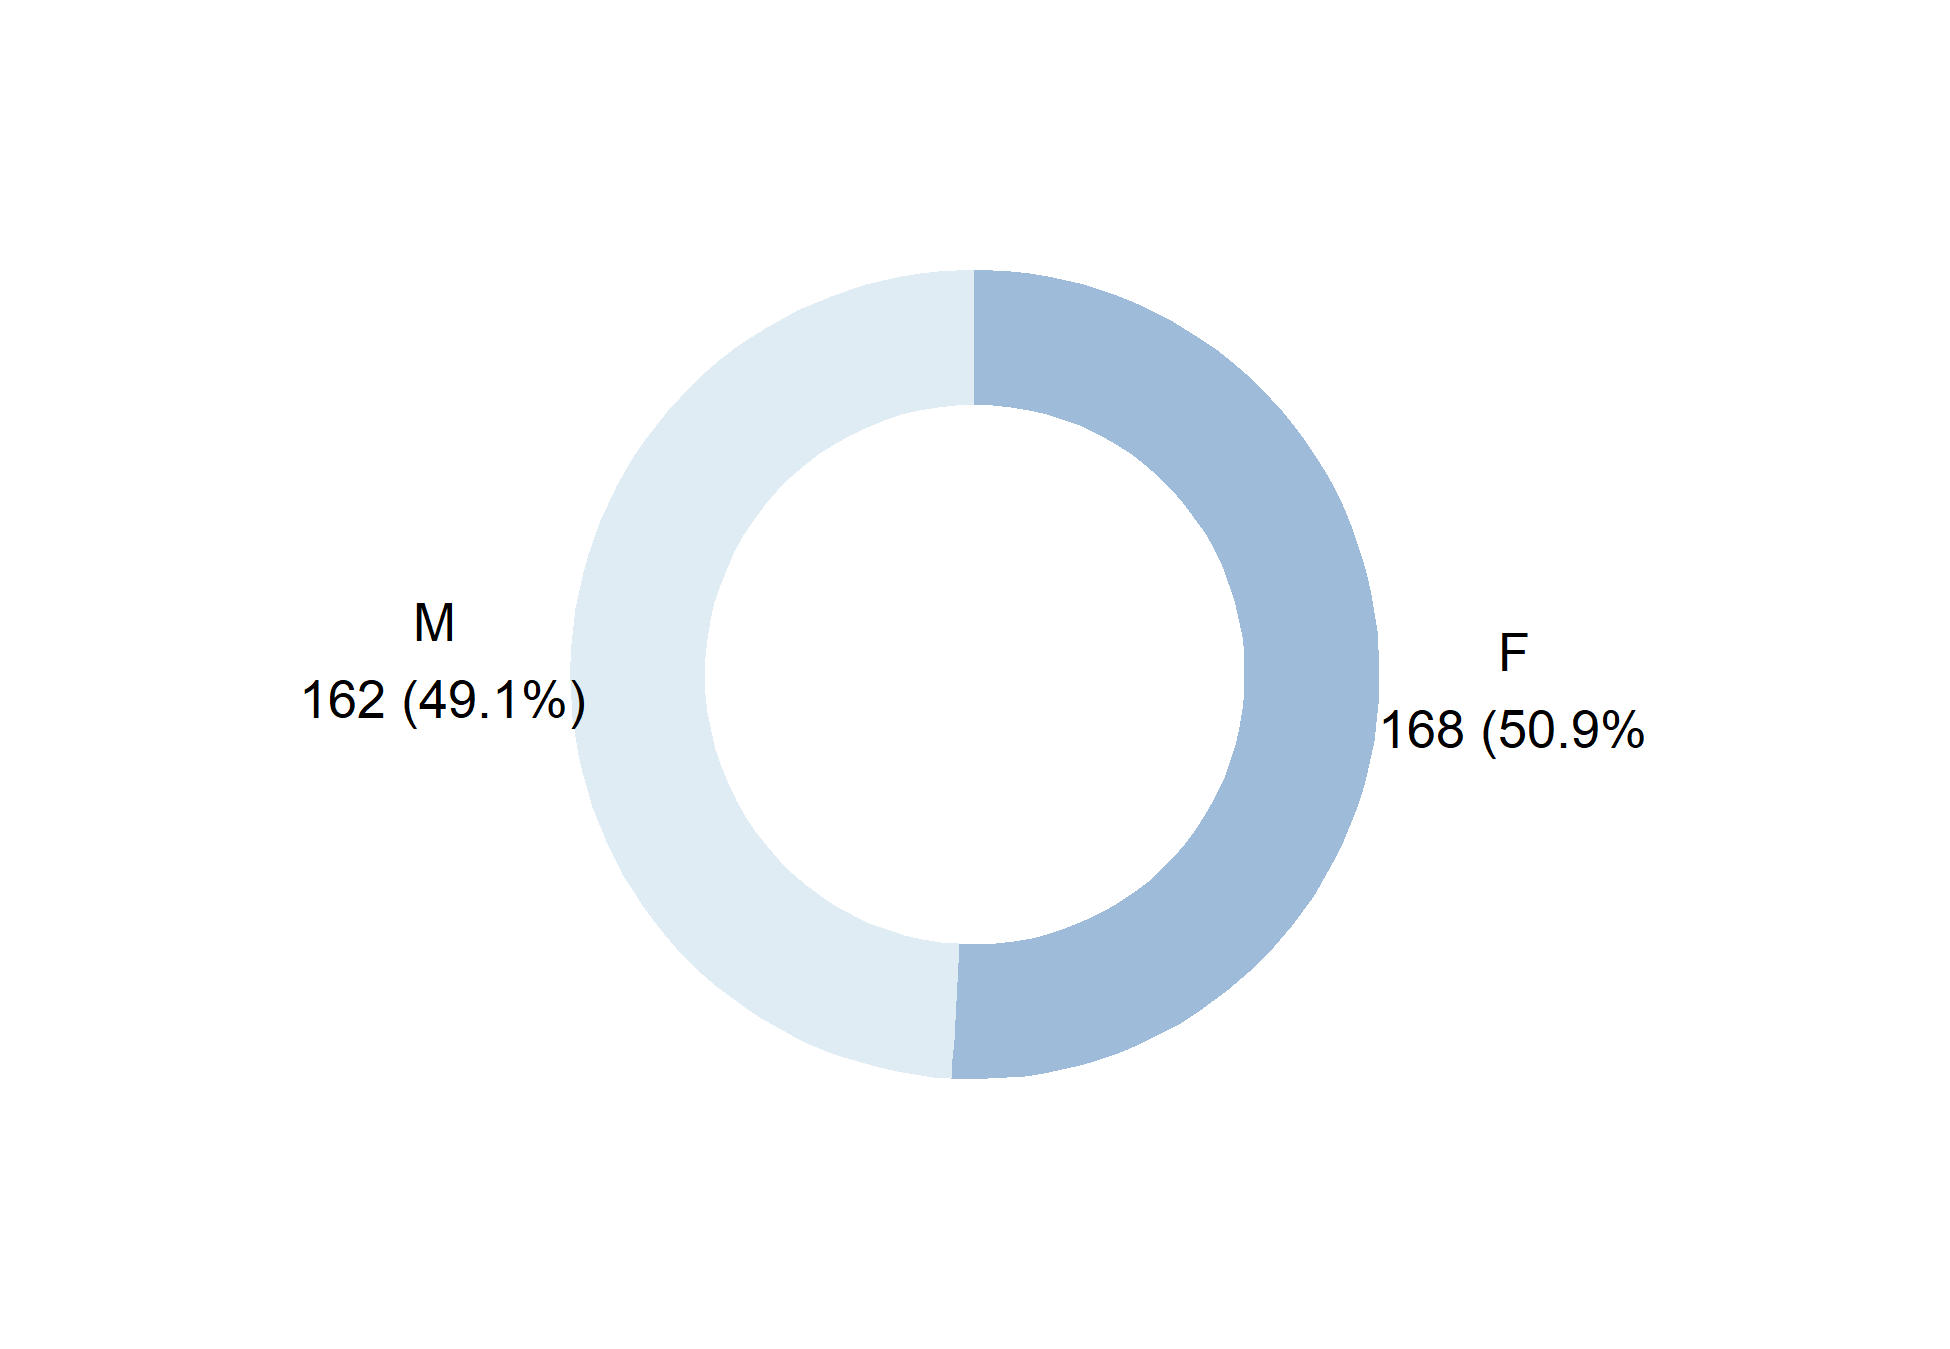
\includegraphics[width=0.7\textwidth]{Imagens/cirurg_SEXO.png}
\end{figure}

\begin{figure}[H]
\caption{Distribuição da queda de acordo com a faixa etária.}
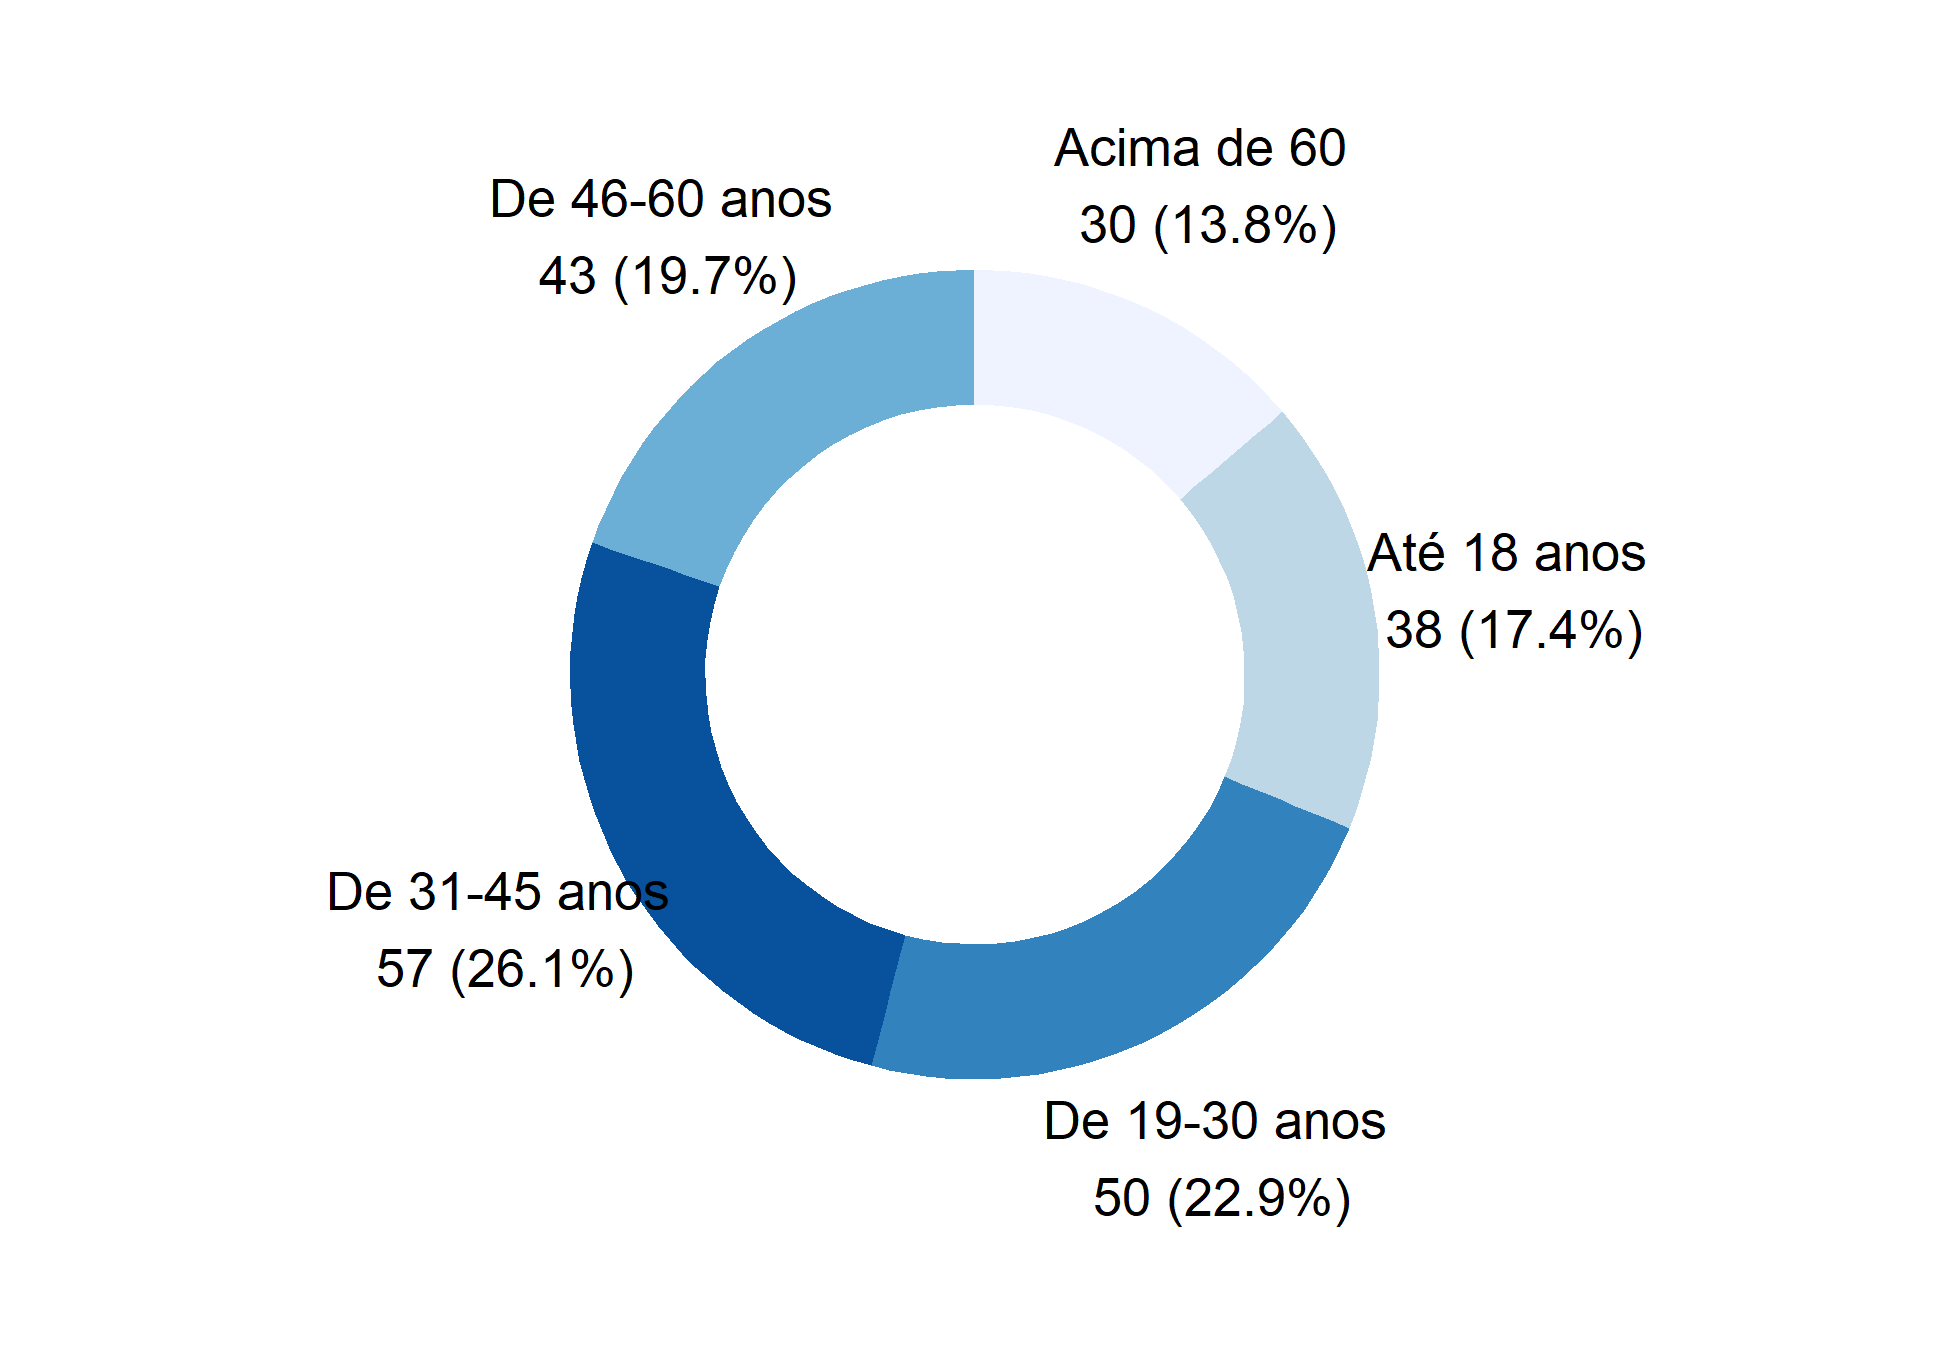
\includegraphics[width=0.7\textwidth]{Imagens/queda_faixa_etaria.png}
\end{figure}

\begin{table}[H]

\caption{\label{tab:unnamed-chunk-8}Dano decorrente da queda (evento adverso)}
\centering
\resizebox{\linewidth}{!}{
\begin{tabular}[t]{lrrr}
\toprule
 & Evento Adverso & Incidente sem dano & Total\\
\midrule
Edema & 5 & 0 & 5\\
Escoriação & 23 & 4 & 27\\
Fratura & 2 & 0 & 2\\
Hematoma & 2 & 2 & 4\\
Hiperemia & 6 & 1 & 7\\
\addlinespace
Lesão corto-contusa & 3 & 0 & 3\\
Outros & 6 & 2 & 8\\
Perda de consciência & 1 & 0 & 1\\
Sem dano & 2 & 159 & 161\\
\midrule
\textbf{Total} & \textbf{50} & \textbf{168} & \textbf{218}\\
\bottomrule
\end{tabular}}
\end{table}

\begin{table}[H]

\caption{\label{tab:unnamed-chunk-9}Motivo da queda.}
\centering
\begin{tabular}[t]{lr}
\toprule
Motivo da Queda & Total\\
\midrule
Perdeu o equilíbrio & 78\\
Escorregou & 49\\
Outros & 46\\
Tropeçou & 13\\
Falha na superfície de apoio (cama-maca, cadeira) & 11\\
\addlinespace
Espasticidade & 7\\
Não observado/Desconhecido & 5\\
Não utilizou auxilio locomoção & 4\\
Síncope & 4\\
Convulsão & 1\\
\midrule
\addlinespace
\textbf{Total} & \textbf{218}\\
\bottomrule
\end{tabular}
\end{table}

\begin{table}[H]

\caption{\label{tab:unnamed-chunk-10}Atividade durante a queda.}
\centering
\begin{tabular}[t]{lr}
\toprule
Atividade & Total\\
\midrule
Locomoção & 53\\
Transferência & 38\\
Outros & 33\\
Higiene & 29\\
Atividade esportiva & 13\\
\addlinespace
Sono/Repouso & 13\\
Reeducação vesico-intestinal & 10\\
Treino de cadeira de rodas & 7\\
Vestuário & 7\\
Treino de marcha & 6\\
\addlinespace
Não observado/Desconhecido & 5\\
Atividade lúdica & 4\\
\midrule
\textbf{Total} & \textbf{218}\\
\bottomrule
\end{tabular}
\end{table}

\begin{table}[H]

\caption{\label{tab:unnamed-chunk-11}Superfície envolvida na queda.}
\centering
\begin{tabular}[t]{lr}
\toprule
Superfície & Total\\
\midrule
Cadeira de rodas & 77\\
Própria altura & 33\\
Cama-maca & 28\\
Auxílio locomoção & 23\\
Cadeira de banho & 22\\
\addlinespace
Outros & 19\\
Cadeira & 6\\
Piso escorregadio & 4\\
Maca & 2\\
Berço & 1\\
\addlinespace
Não observado/Desconhecido & 1\\
Piso solto & 1\\
Transferidor de paciente & 1\\
\midrule
\textbf{Total} & \textbf{218}\\
\bottomrule
\end{tabular}
\end{table}

\subsection{Lesão por Pressão (LP)}

\begin{table}[H]

\caption{\label{tab:unnamed-chunk-12}Tipo de Lesão por Pressão.}
\centering
\resizebox{\linewidth}{!}{
\begin{tabular}[t]{lrrrrrrrrrrrr}
\toprule
 & jan & fev & mar & abr & mai & jun & jul & ago & set & out & nov & Total\\
\midrule
Em membranas mucosas & 2 & 0 & 2 & 0 & 1 & 0 & 3 & 1 & 1 & 1 & 1 & 12\\
Em proeminências ósseas & 8 & 6 & 3 & 4 & 6 & 3 & 5 & 5 & 10 & 6 & 4 & 60\\
Relacionada a dispositivo médico & 3 & 4 & 6 & 5 & 8 & 4 & 4 & 11 & 10 & 7 & 4 & 66\\
\midrule
\textbf{Total} & \textbf{13} & \textbf{10} & \textbf{11} & \textbf{9} & \textbf{15} & \textbf{7} & \textbf{12} & \textbf{17} & \textbf{21} & \textbf{14} & \textbf{9} & \textbf{138}\\
\bottomrule
\end{tabular}}
\end{table}

\subsubsection{Lesão por Pressão em Proeminência Óssea}

\begin{table}[H]

\caption{\label{tab:unnamed-chunk-13}Tipo de LP em proeminência óssea}
\centering
\begin{tabular}[t]{lr}
\toprule
Tipo & Total\\
\midrule
Primária & 31\\
Por posicionamento cirúrgico & 25\\
Sobre cicatriz prévia & 12\\
\midrule
\textbf{Total} & \textbf{68}\\
\bottomrule
\end{tabular}
\end{table}

\begin{figure}[H]
\caption{Faixa etária dos pacientes com LP primária em proeminência óssea.}
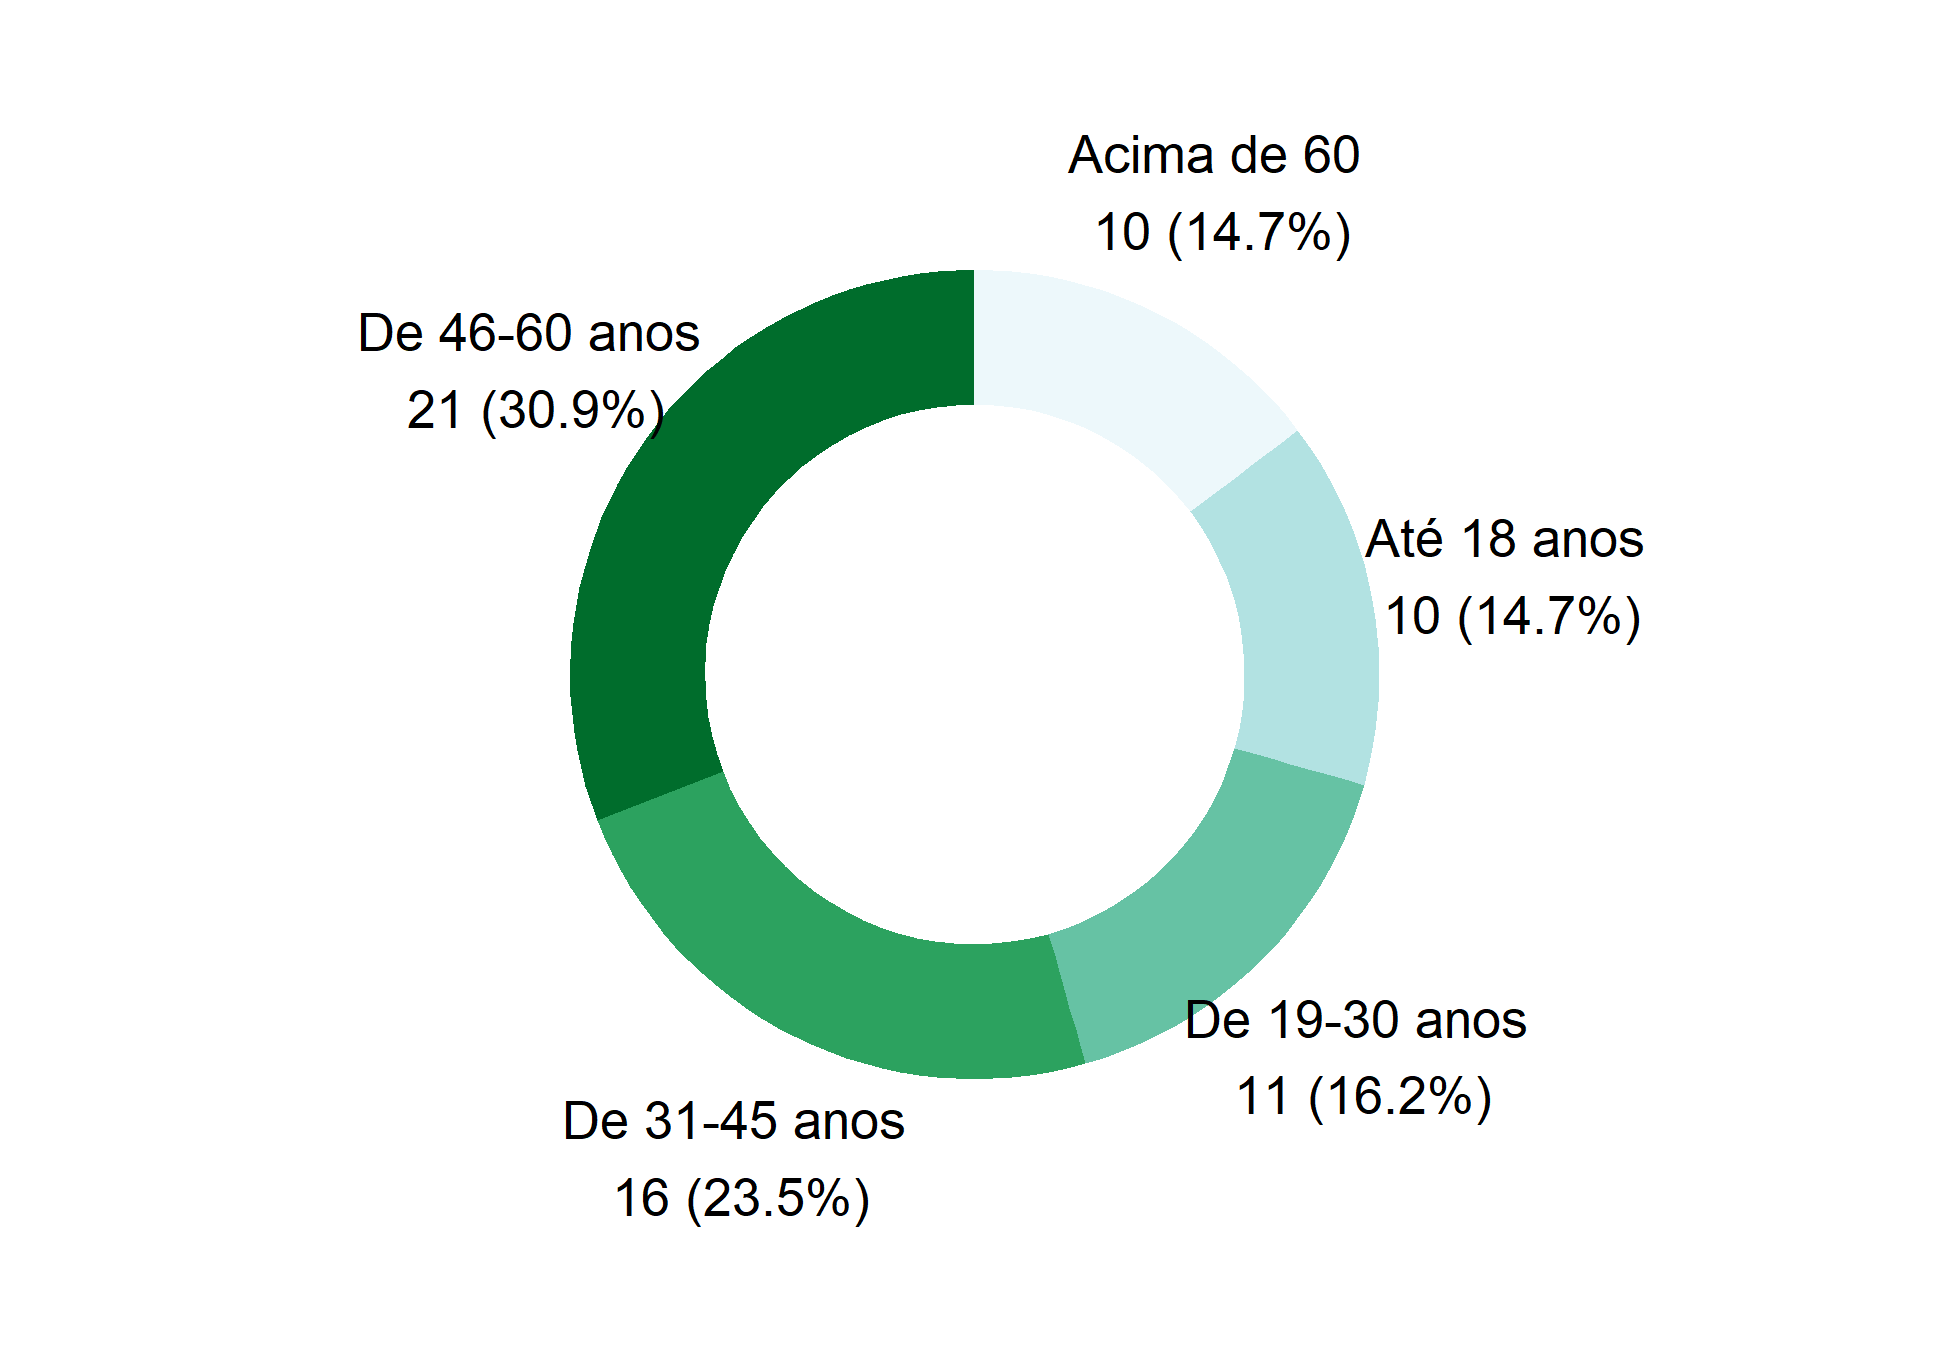
\includegraphics[width=0.7\textwidth]{Imagens/lesao_pressao_faixa_etaria.png}
\end{figure}

\begin{figure}[H]
\caption{Sexo dos pacientes com LP primária em proeminência óssea.}
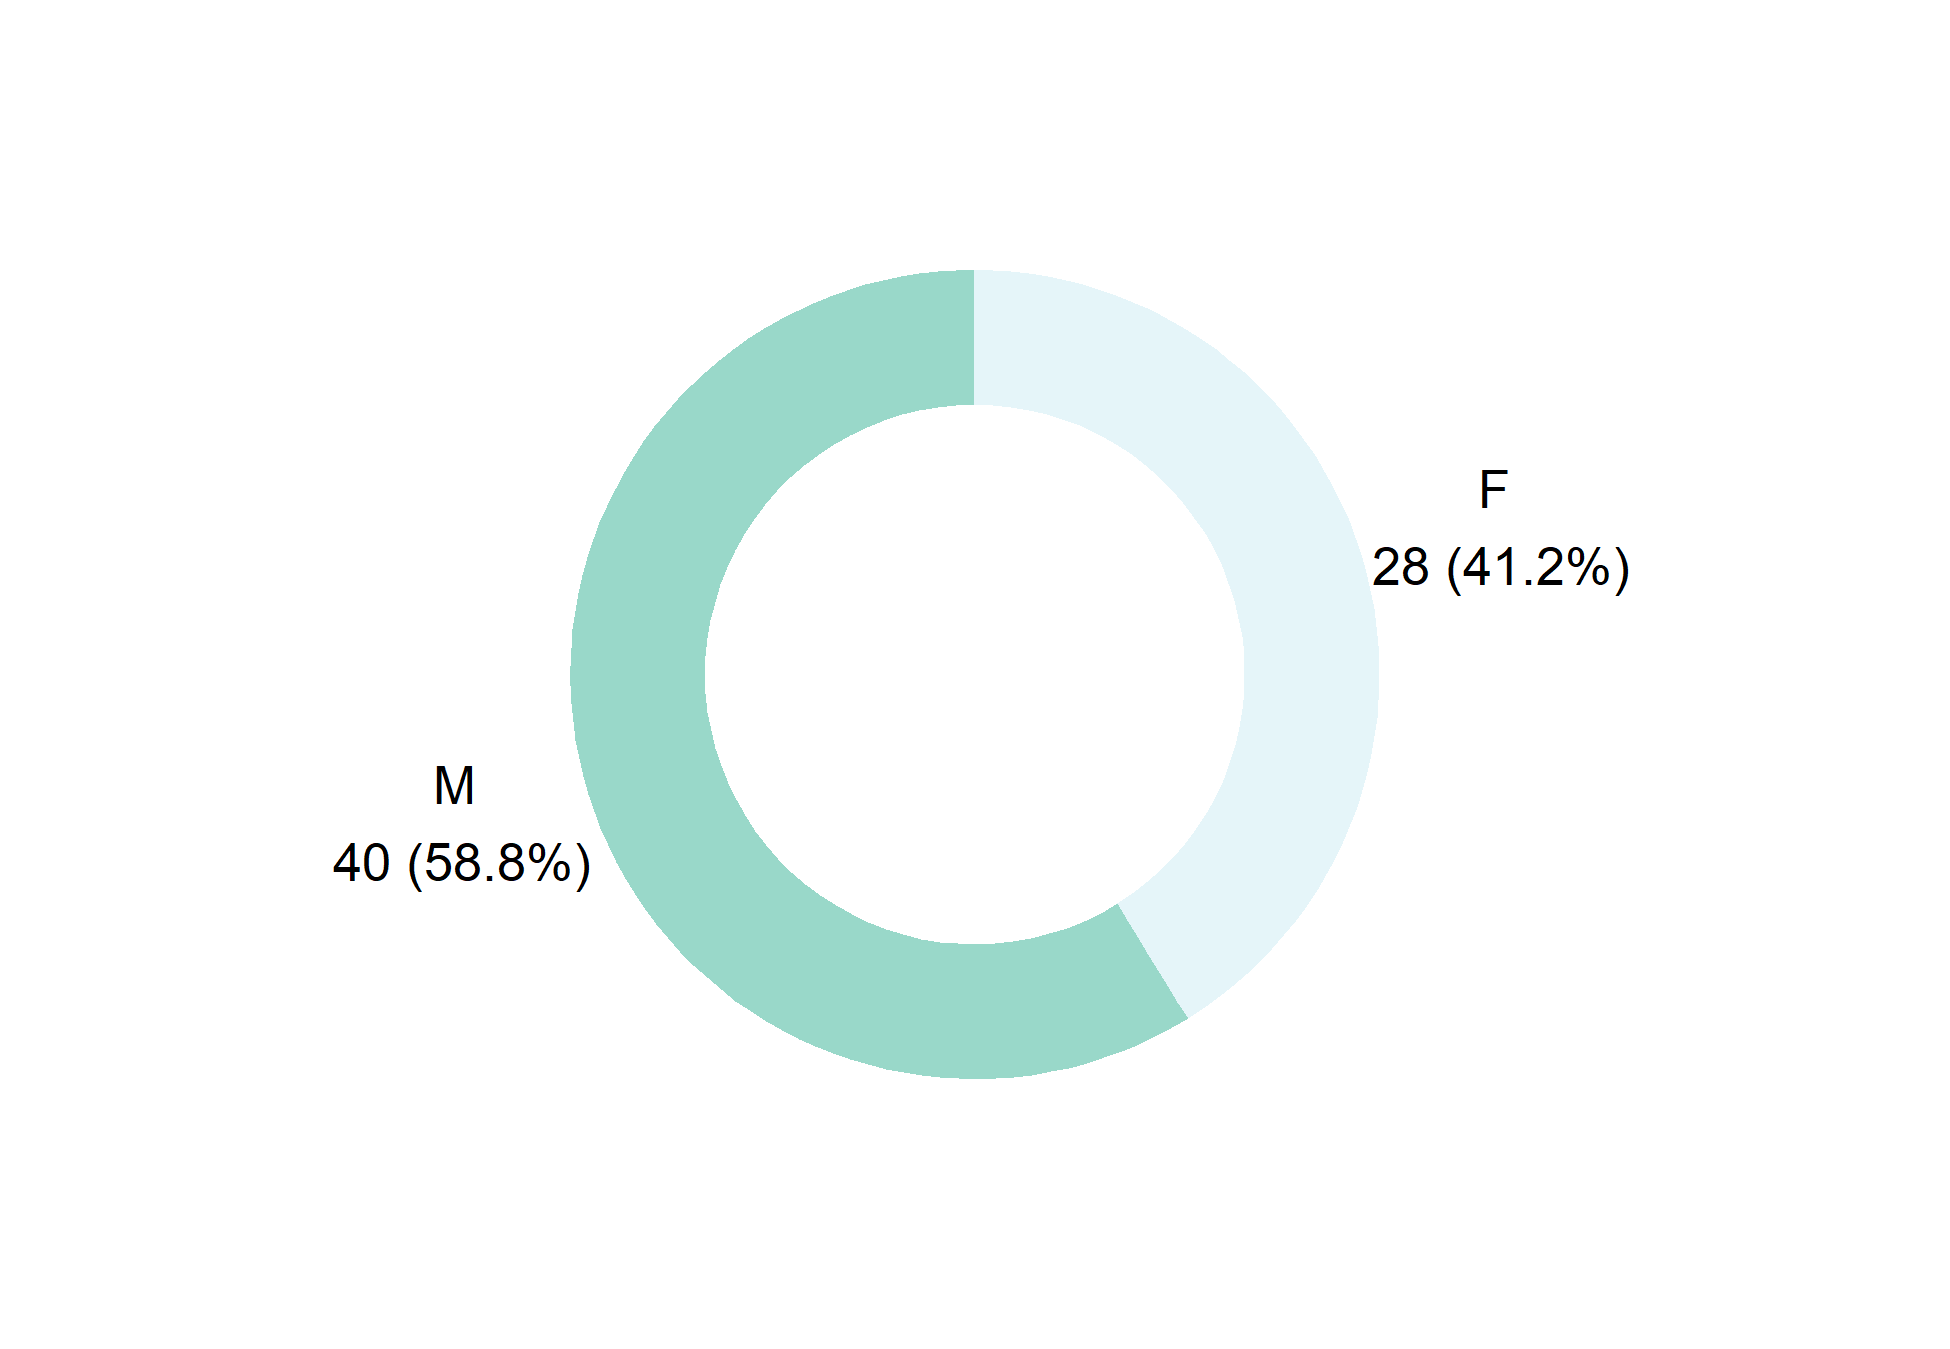
\includegraphics[width=0.7\textwidth]{Imagens/lesao_pressao_sexo.png}
\end{figure}

\begin{table}[H]

\caption{\label{tab:unnamed-chunk-16}Comprometimento tissular da LP primária em proeminência óssea}
\centering
\begin{tabular}[t]{lr}
\toprule
Comprometimento tissular & Total\\
\midrule
Estágio 1 & 40\\
Estágio 2 & 25\\
Lesão tissular profunda & 2\\
Estágio 3 & 1\\
\midrule
\textbf{Total} & \textbf{68}\\
\bottomrule
\end{tabular}
\end{table}

\begin{table}[H]

\caption{\label{tab:unnamed-chunk-17}Localização da LP primária em proeminência óssea}
\centering
\begin{tabular}[t]{lr}
\toprule
PO - Localização da lesão & Total\\
\midrule
Sacro & 21\\
Calcâneo & 11\\
Mento & 5\\
Ísquio & 4\\
Região torácica lateral & 4\\
\addlinespace
Pavilhão auditivo & 3\\
Epicôndilo medial (fêmur) & 2\\
Fronte & 2\\
Fronte
Mento & 2\\
Processo espinhoso & 2\\
\addlinespace
Trocânter & 2\\
Crista ilíaca anterior & \vphantom{1} 1\\
Crista ilíaca posterior & 1\\
Epicôndilo lateral (úmero) & 1\\
Maléolo lateral & 1\\
\addlinespace
Mento
Fronte & 1\\
Mento
Fronte
Crista ilíaca anterior & 1\\
Olécrano & 1\\
Patela & 1\\
Região occiptal & 1\\
\addlinespace
Zigomático & 1\\
\midrule
\textbf{Total} & \textbf{68}\\
\bottomrule
\end{tabular}
\end{table}

\subsubsection{Lesão por Pressão relacionada ao dispositivo médico}

\begin{table}[H]

\caption{\label{tab:unnamed-chunk-18}Comprometimento tissular da LP relacionada ao dispositivo médico}
\centering
\begin{tabular}[t]{lr}
\toprule
Comprometimento tissular & Total\\
\midrule
Estágio 2 & 34\\
Estágio 1 & 20\\
Não classificável & 9\\
Lesão tissular profunda & 5\\
Estágio 3 & 4\\
\addlinespace
Estágio 4 & 1\\
\midrule
\textbf{Total} & \textbf{73}\\
\bottomrule
\end{tabular}
\end{table}

\begin{table}[H]

\caption{\label{tab:unnamed-chunk-19}Localização da LP relacionada ao dispositivo médico}
\centering
\begin{tabular}[t]{lr}
\toprule
DM - Localização da lesão. & Total\\
\midrule
Calcâneo & 29\\
Patela & 11\\
Maléolo lateral & 6\\
Pavilhão auditivo & 6\\
coxa & 5\\
\addlinespace
Flanco & 3\\
Projeção medial dos metatarsos & 3\\
Corpo nasal & 2\\
Antebraço & 1\\
Braço & 1\\
\addlinespace
Crista ilíaca anterior & 1\\
Fronte & 1\\
Maléolo medial & 1\\
Projeção lateral dos metatarsos & 1\\
Região cervical & 1\\
\addlinespace
Zigomático & 1\\
\midrule
\textbf{Total} & \textbf{73}\\
\bottomrule
\end{tabular}
\end{table}

\begin{table}[H]

\caption{\label{tab:unnamed-chunk-20}Dispositivo médico relacionado a LP}
\centering
\begin{tabular}[t]{lr}
\toprule
Dispositivo & Total\\
\midrule
Gesso & 36\\
Outros & 22\\
Órtese de locomoção & 7\\
Órtese de posicionamento & 5\\
Cadarço de traqueostomia & 1\\
\addlinespace
Colete & 1\\
Fixador externo & 1\\
\midrule
\textbf{Total} & \textbf{73}\\
\bottomrule
\end{tabular}
\end{table}

\subsection{Lesão Traumática}

\begin{figure}[H]
\caption{Distribuição do gênero nas notificações em Procedimento Cirúrgico.}
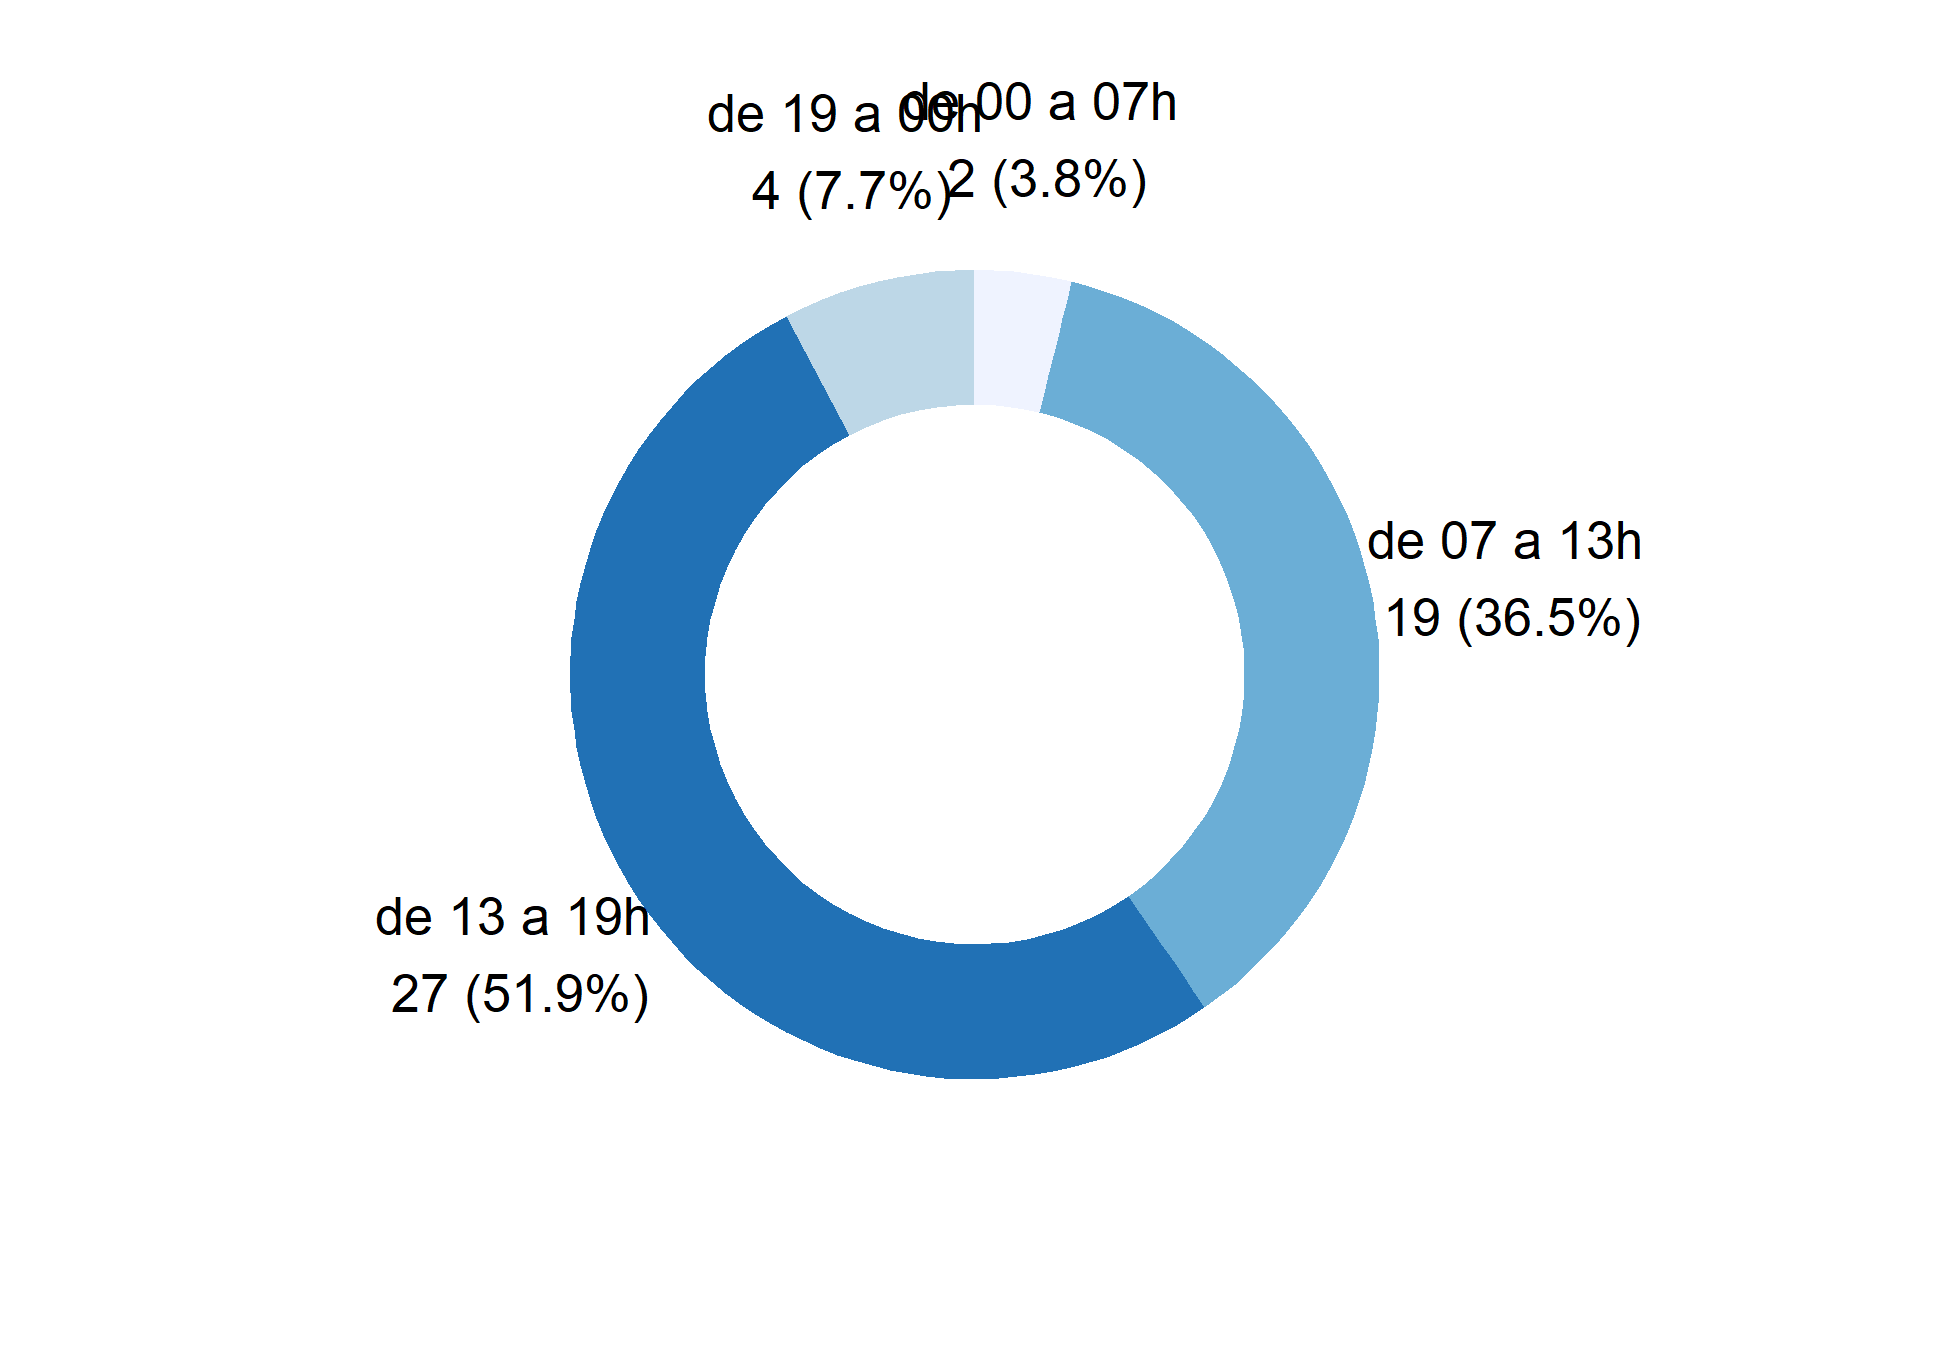
\includegraphics[width=0.7\textwidth]{Imagens/trauma_periodo.png}
\end{figure}

\begin{figure}[H]
\caption{Distribuição do gênero nas notificações em Procedimento Cirúrgico.}
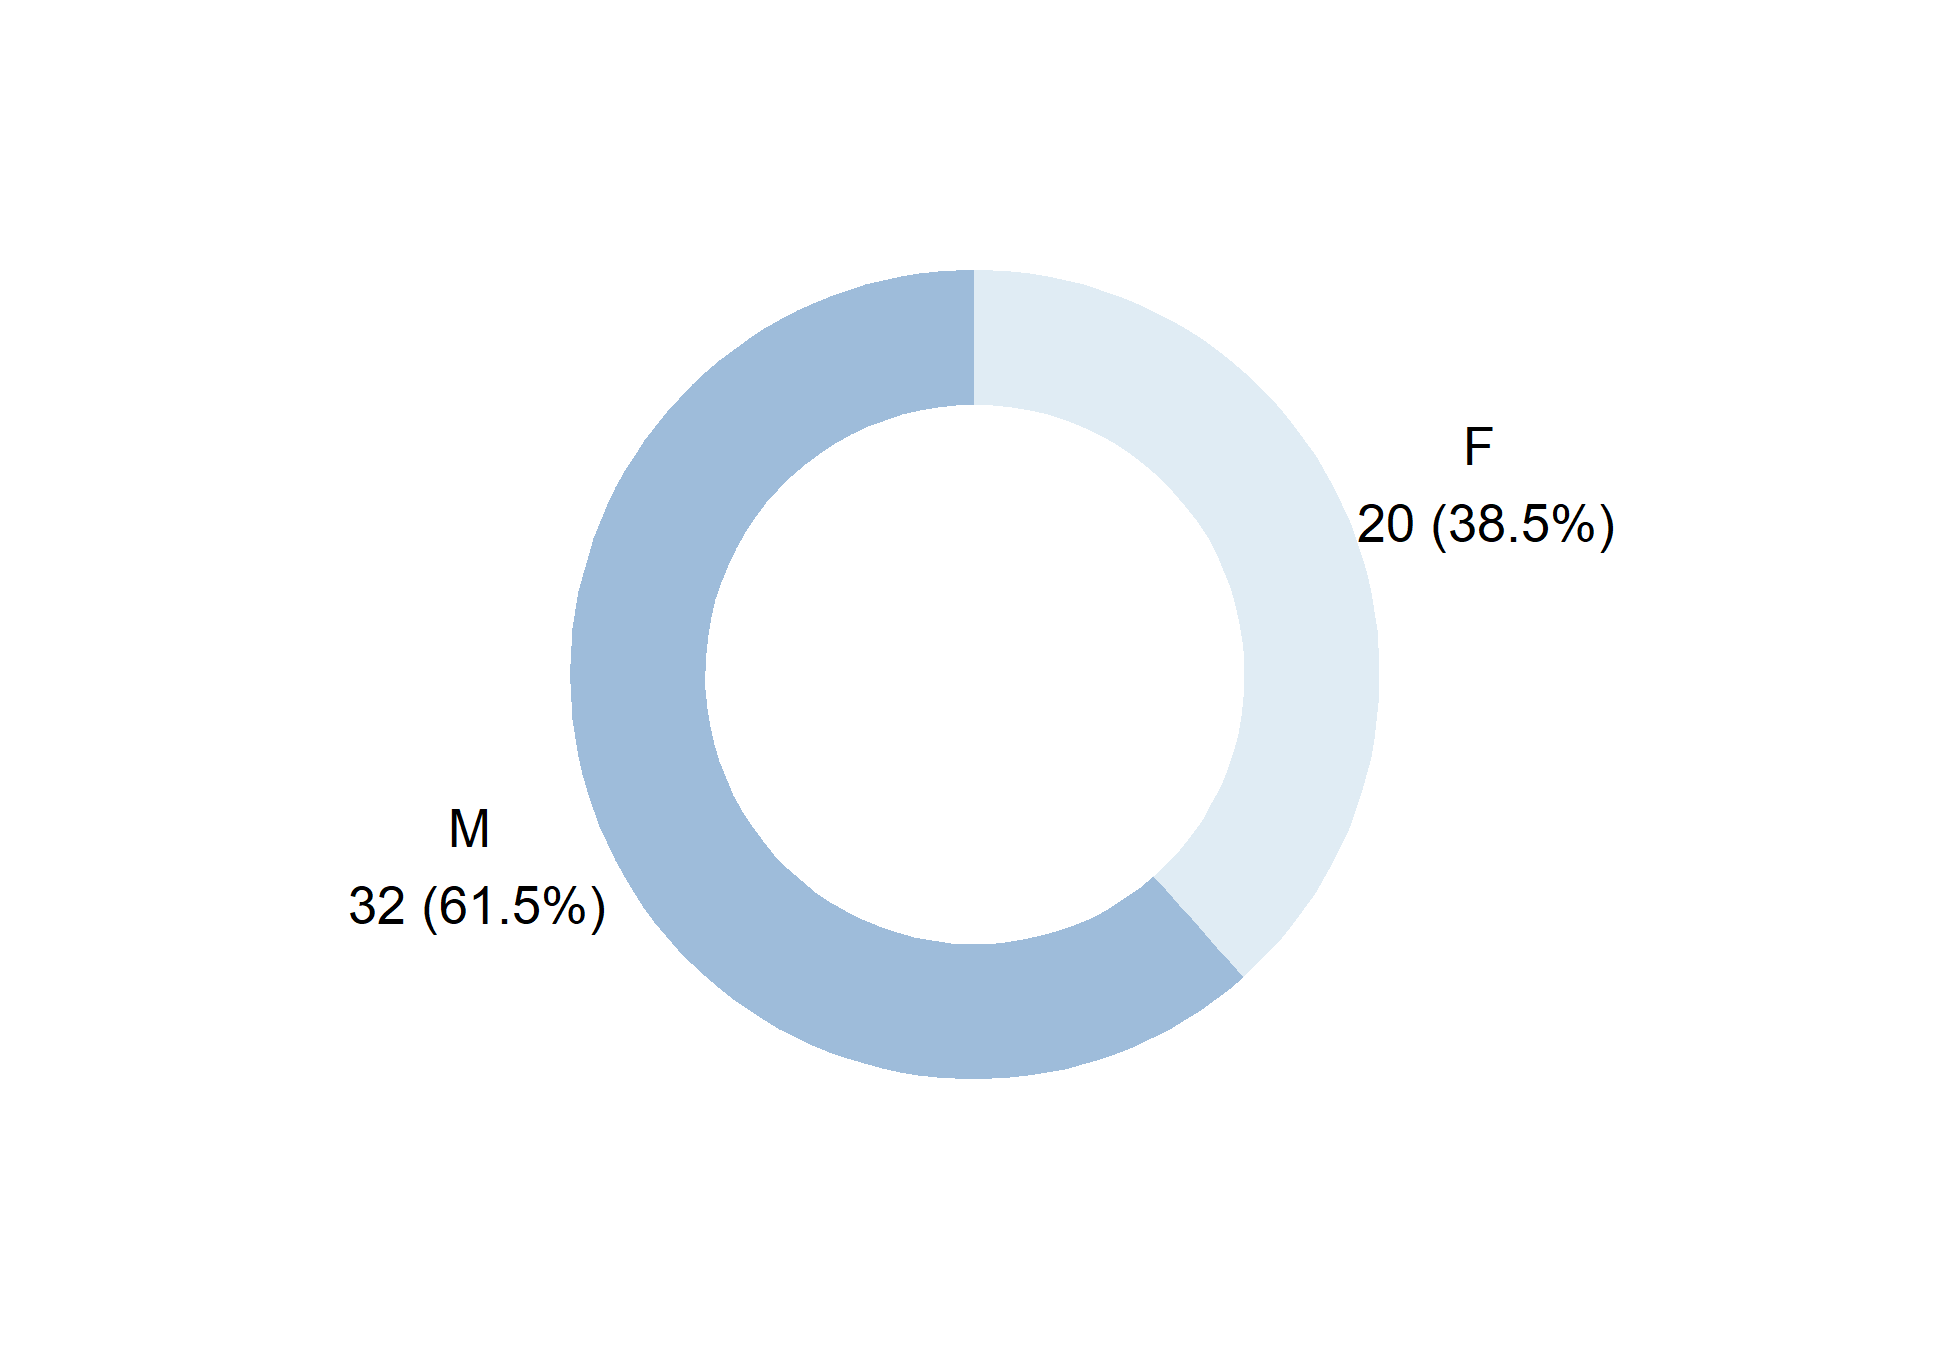
\includegraphics[width=0.7\textwidth]{Imagens/trauma_SEXO.png}
\end{figure}

\begin{figure}[H]
\caption{Distribuição da queda de acordo com a faixa etária.}
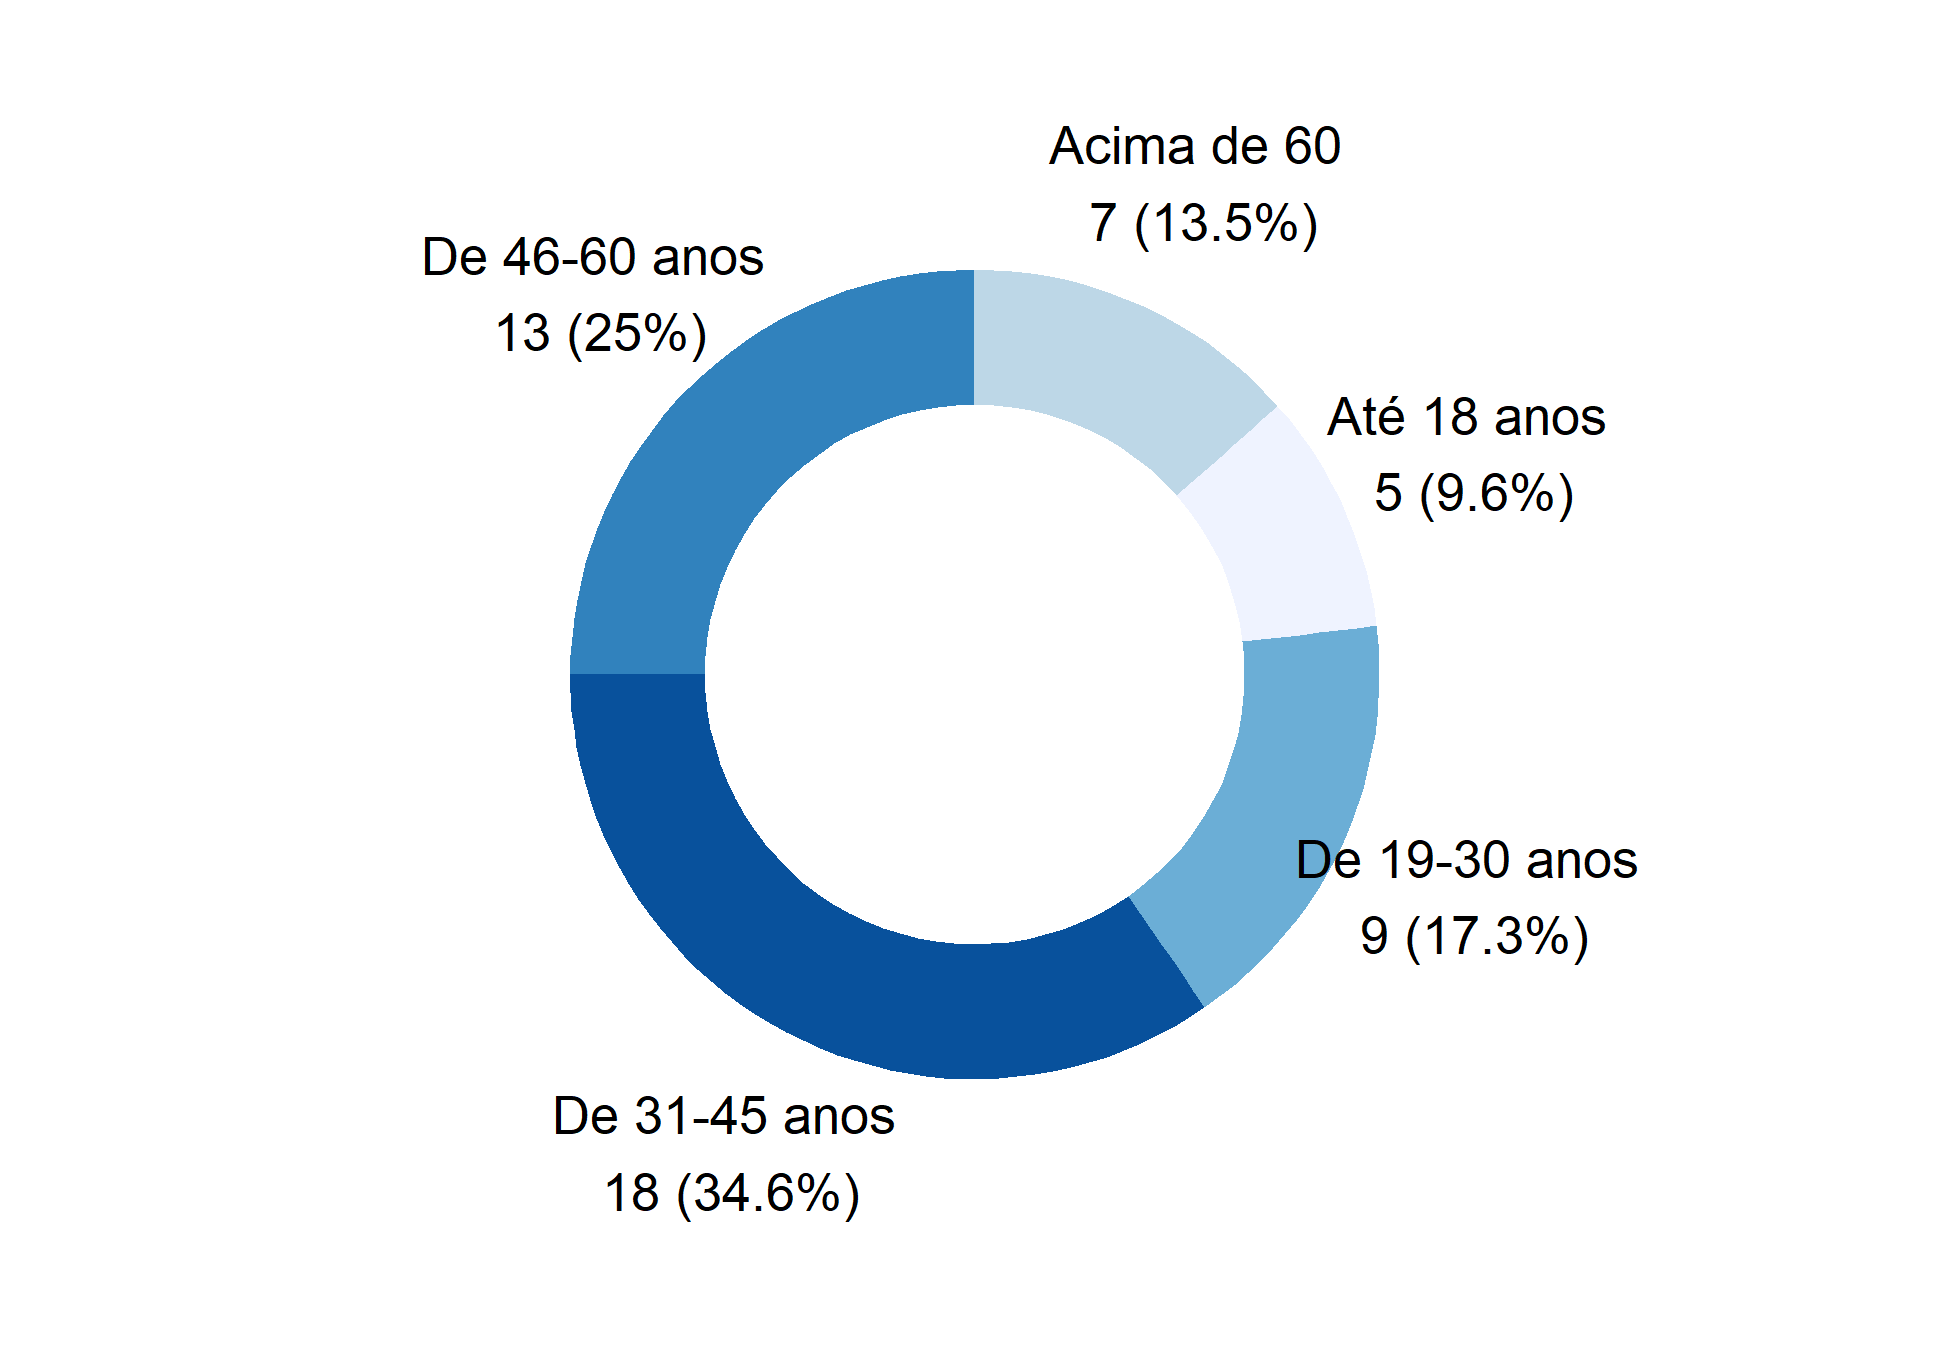
\includegraphics[width=0.7\textwidth]{Imagens/trauma_faixa_etaria.png}
\end{figure}

\begin{table}[H]

\caption{\label{tab:unnamed-chunk-24}Tipo de Lesão Traumática}
\centering
\resizebox{\linewidth}{!}{
\begin{tabular}[t]{lrrrrrrrrrrrr}
\toprule
 & jan & fev & mar & abr & mai & jun & jul & ago & set & out & nov & Total\\
\midrule
Abrasão & 3 & 1 & 2 & 0 & 0 & 0 & 1 & 2 & 0 & 0 & 1 & 10\\
Arranhadura & 1 & 0 & 1 & 0 & 0 & 0 & 0 & 0 & 0 & 0 & 0 & 2\\
Corte-contusa & 3 & 3 & 1 & 0 & 0 & 0 & 0 & 0 & 1 & 2 & 3 & 13\\
Escoriação & 3 & 1 & 3 & 3 & 0 & 1 & 3 & 2 & 4 & 1 & 1 & 22\\
Skin Tears (fricção) & 0 & 0 & 0 & 0 & 1 & 0 & 1 & 0 & 0 & 0 & 0 & 2\\
\midrule
\addlinespace
\textbf{Total} & \textbf{10} & \textbf{5} & \textbf{7} & \textbf{3} & \textbf{1} & \textbf{1} & \textbf{5} & \textbf{4} & \textbf{5} & \textbf{3} & \textbf{5} & \textbf{49}\\
\bottomrule
\end{tabular}}
\end{table}

\begin{table}[H]

\caption{\label{tab:unnamed-chunk-25}Atividade envolvida na lesão traumática}
\centering
\begin{tabular}[t]{lr}
\toprule
Atividade & Total\\
\midrule
Outros procedimentos (curativo, gesso, etc) & 14\\
Transferências (cama-cadeira; cadeira-sanitário, outros) & 10\\
Procedimento cirúrgico & 8\\
Atividade esportiva & 5\\
Treino de habilidades com cadeira & 4\\
\addlinespace
Uso de fixadores externos & 4\\
Mudança de decúbito & 2\\
Realização de exames & 2\\
Treino de marcha & 2\\
Canoagem & 1\\
\midrule
\addlinespace
\textbf{Total} & \textbf{52}\\
\bottomrule
\end{tabular}
\end{table}

\subsection{Lesão de Pele}

\begin{figure}[H]
\caption{Distribuição do horário do incidente em Lesão de pele}
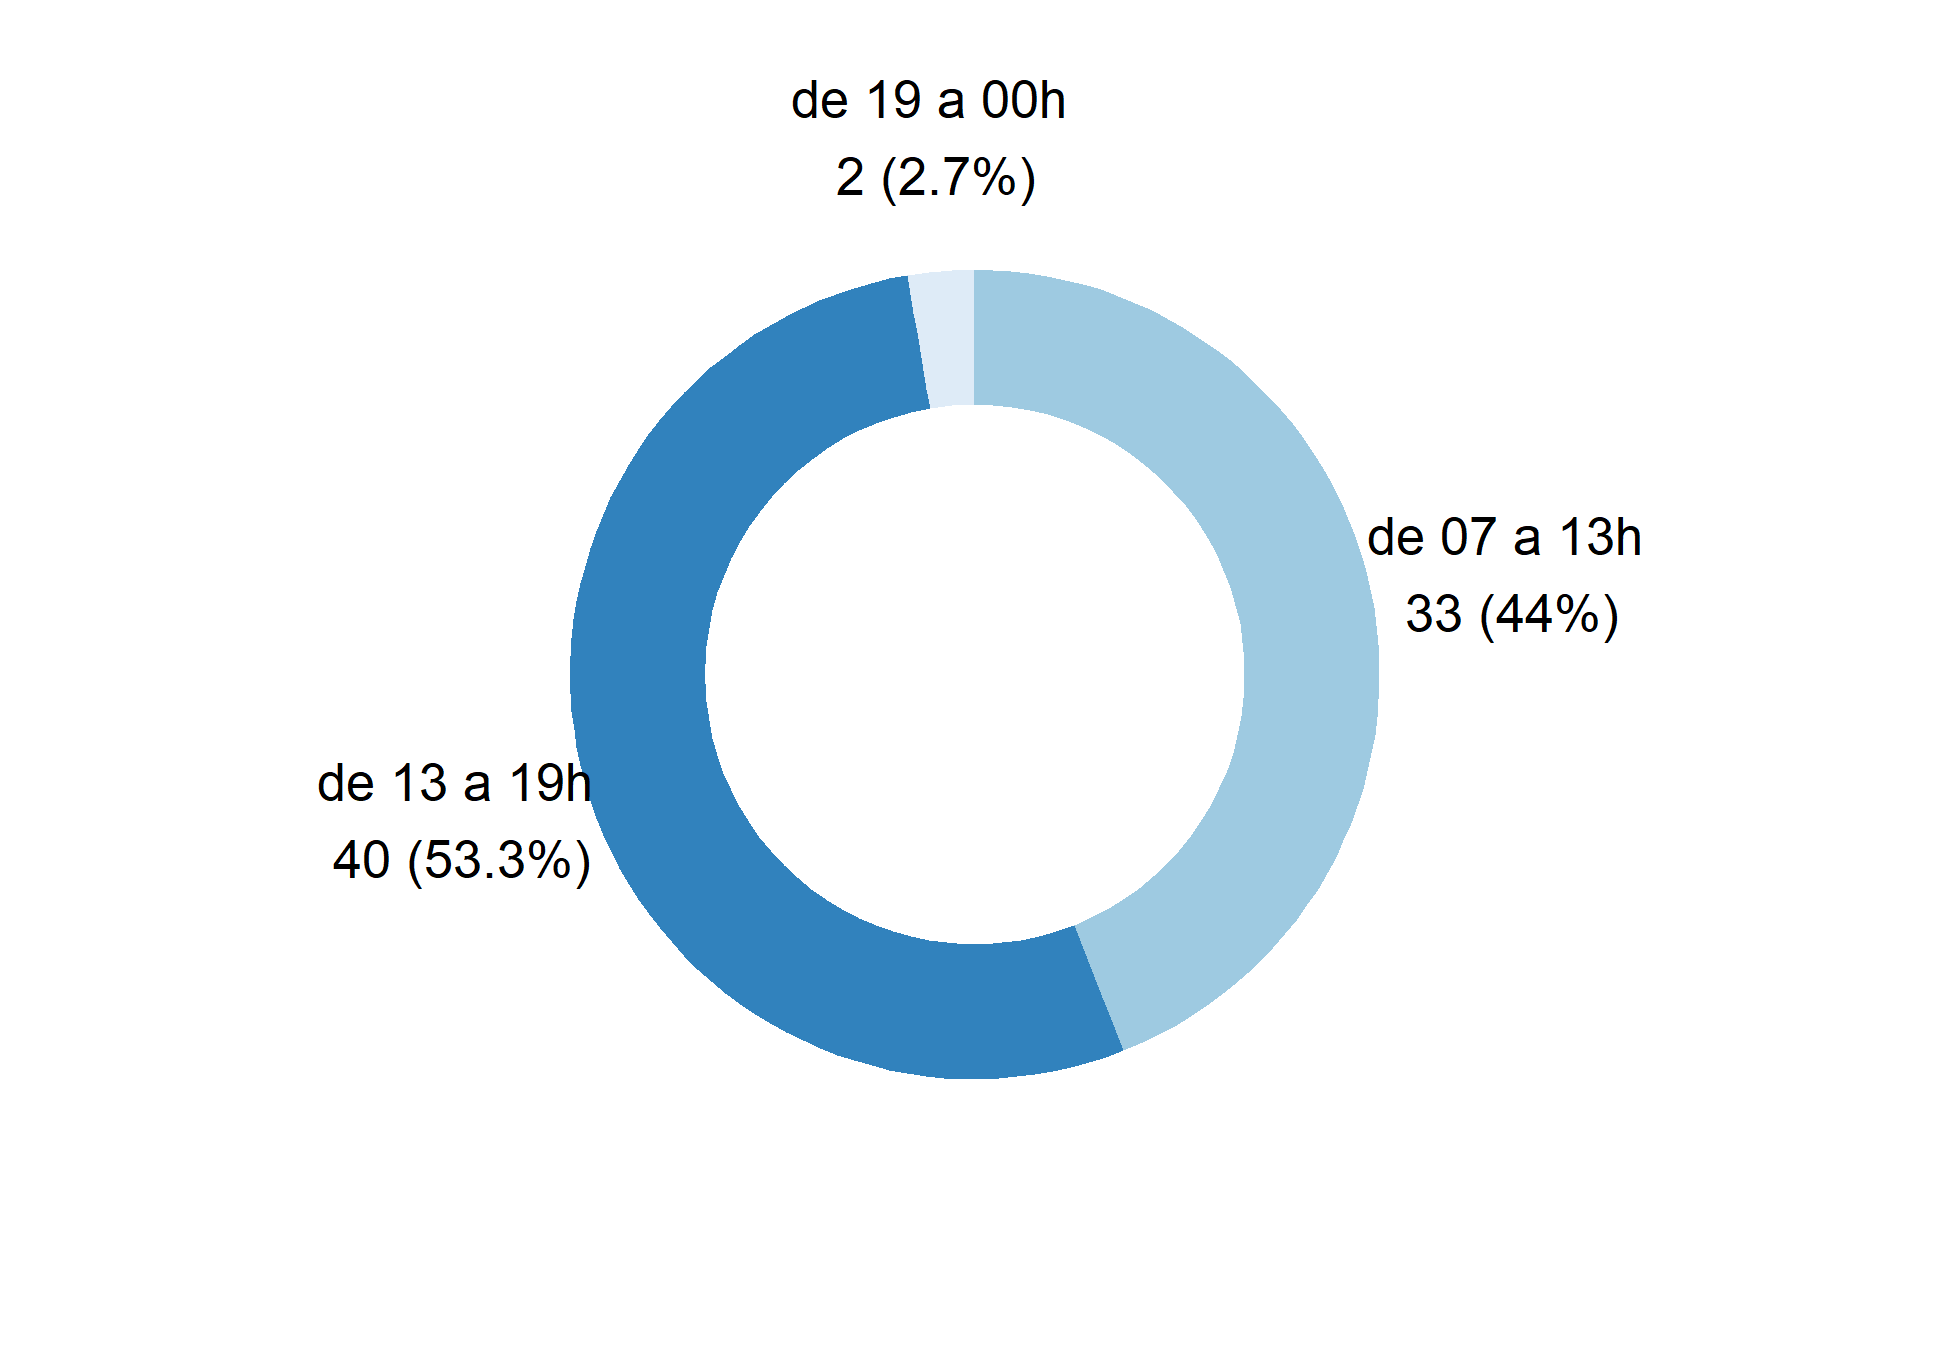
\includegraphics[width=0.7\textwidth]{Imagens/pele_periodo.png}
\end{figure}

\begin{figure}[H]
\caption{Distribuição do gênero nas notificações em Lesão de pele}
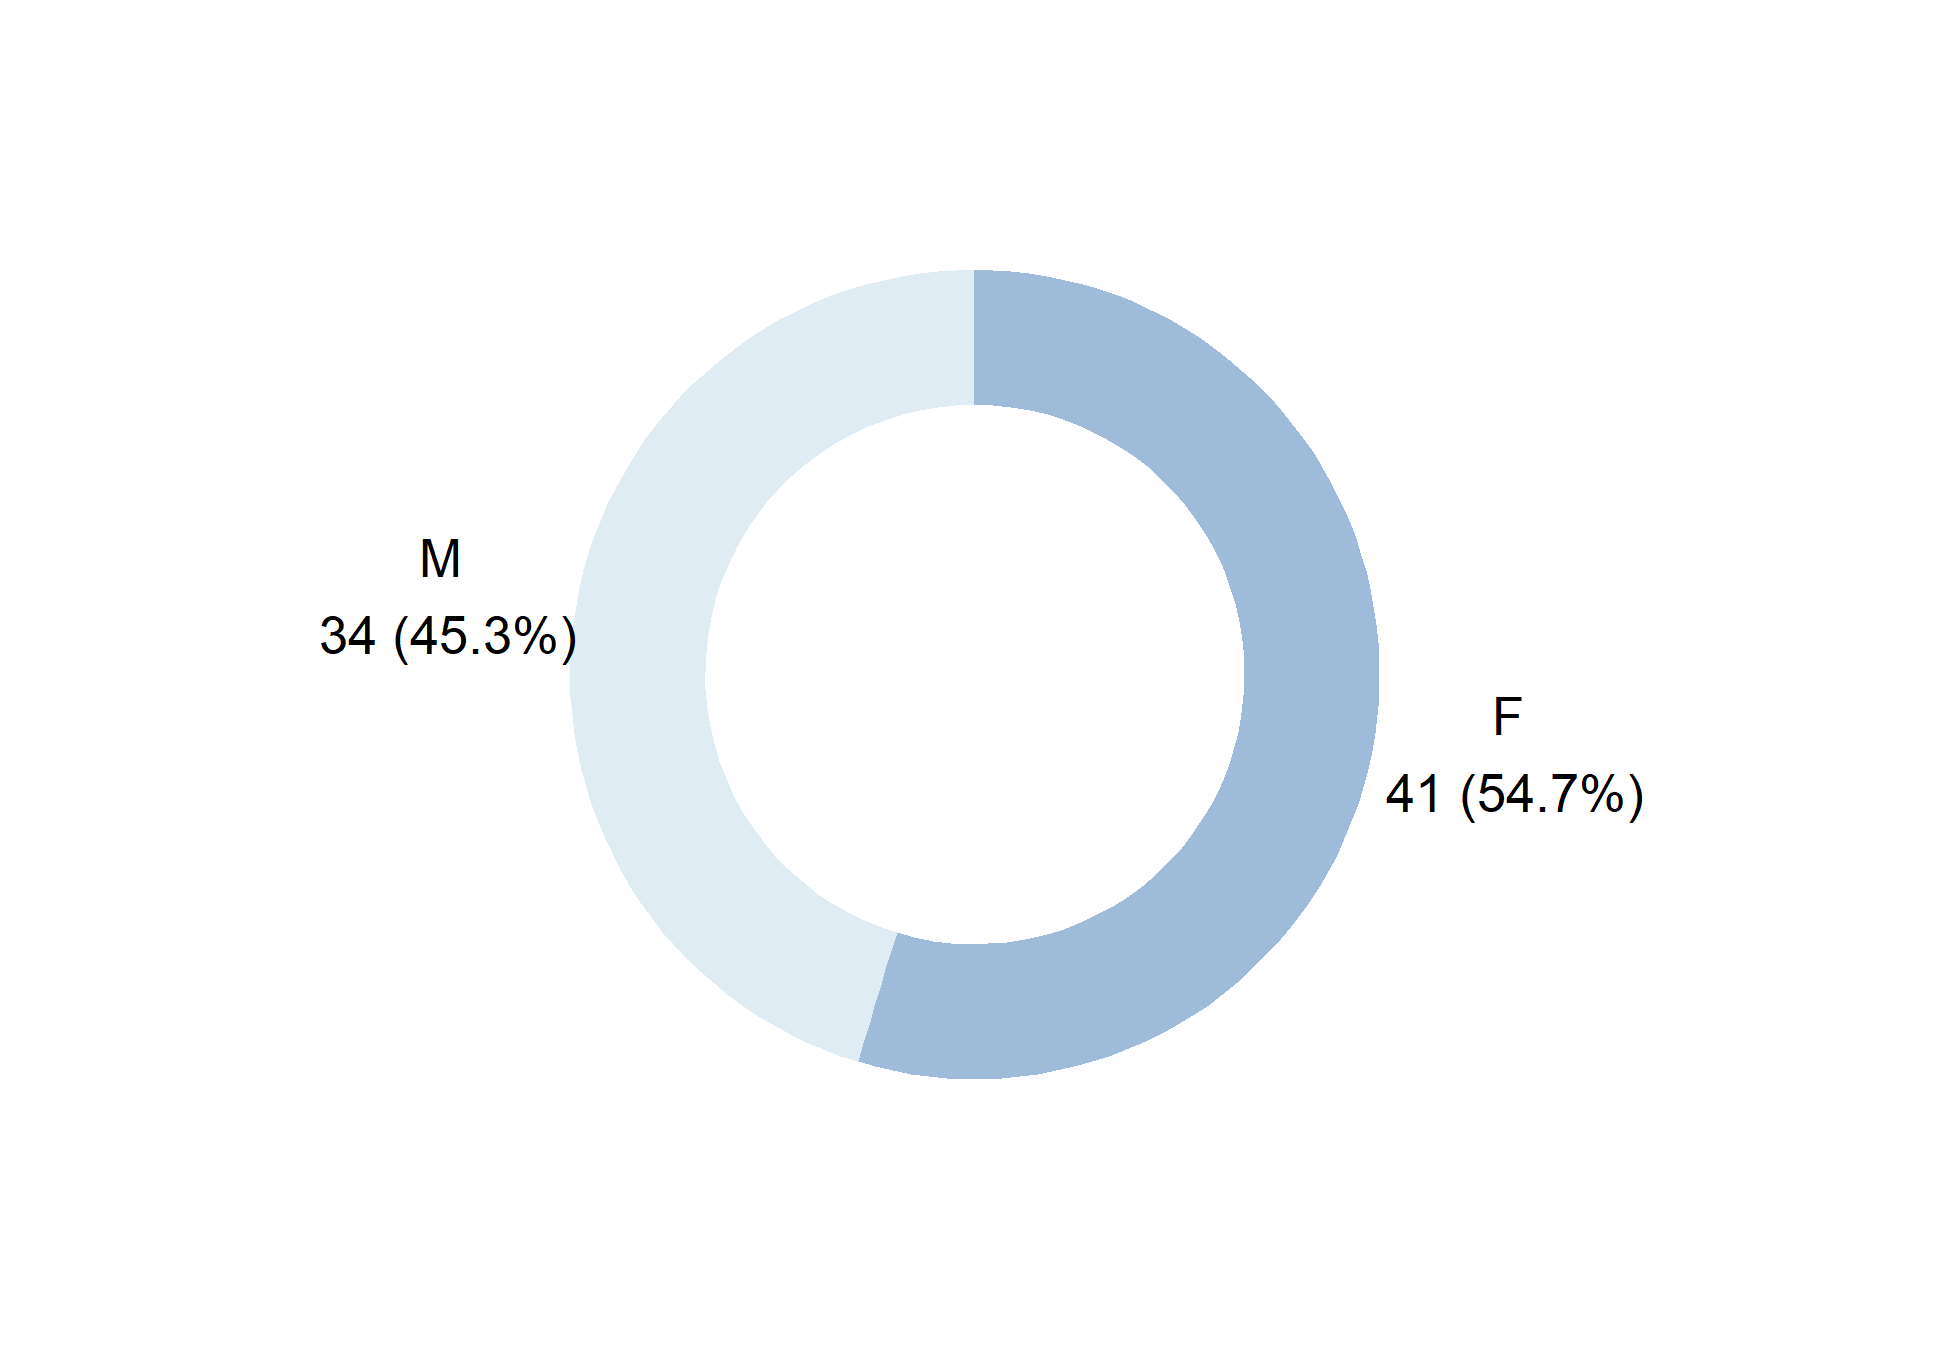
\includegraphics[width=0.7\textwidth]{Imagens/pele_SEXO.png}
\end{figure}

\begin{figure}[H]
\caption{Distribuição da faixa etária em Lesão por pele}
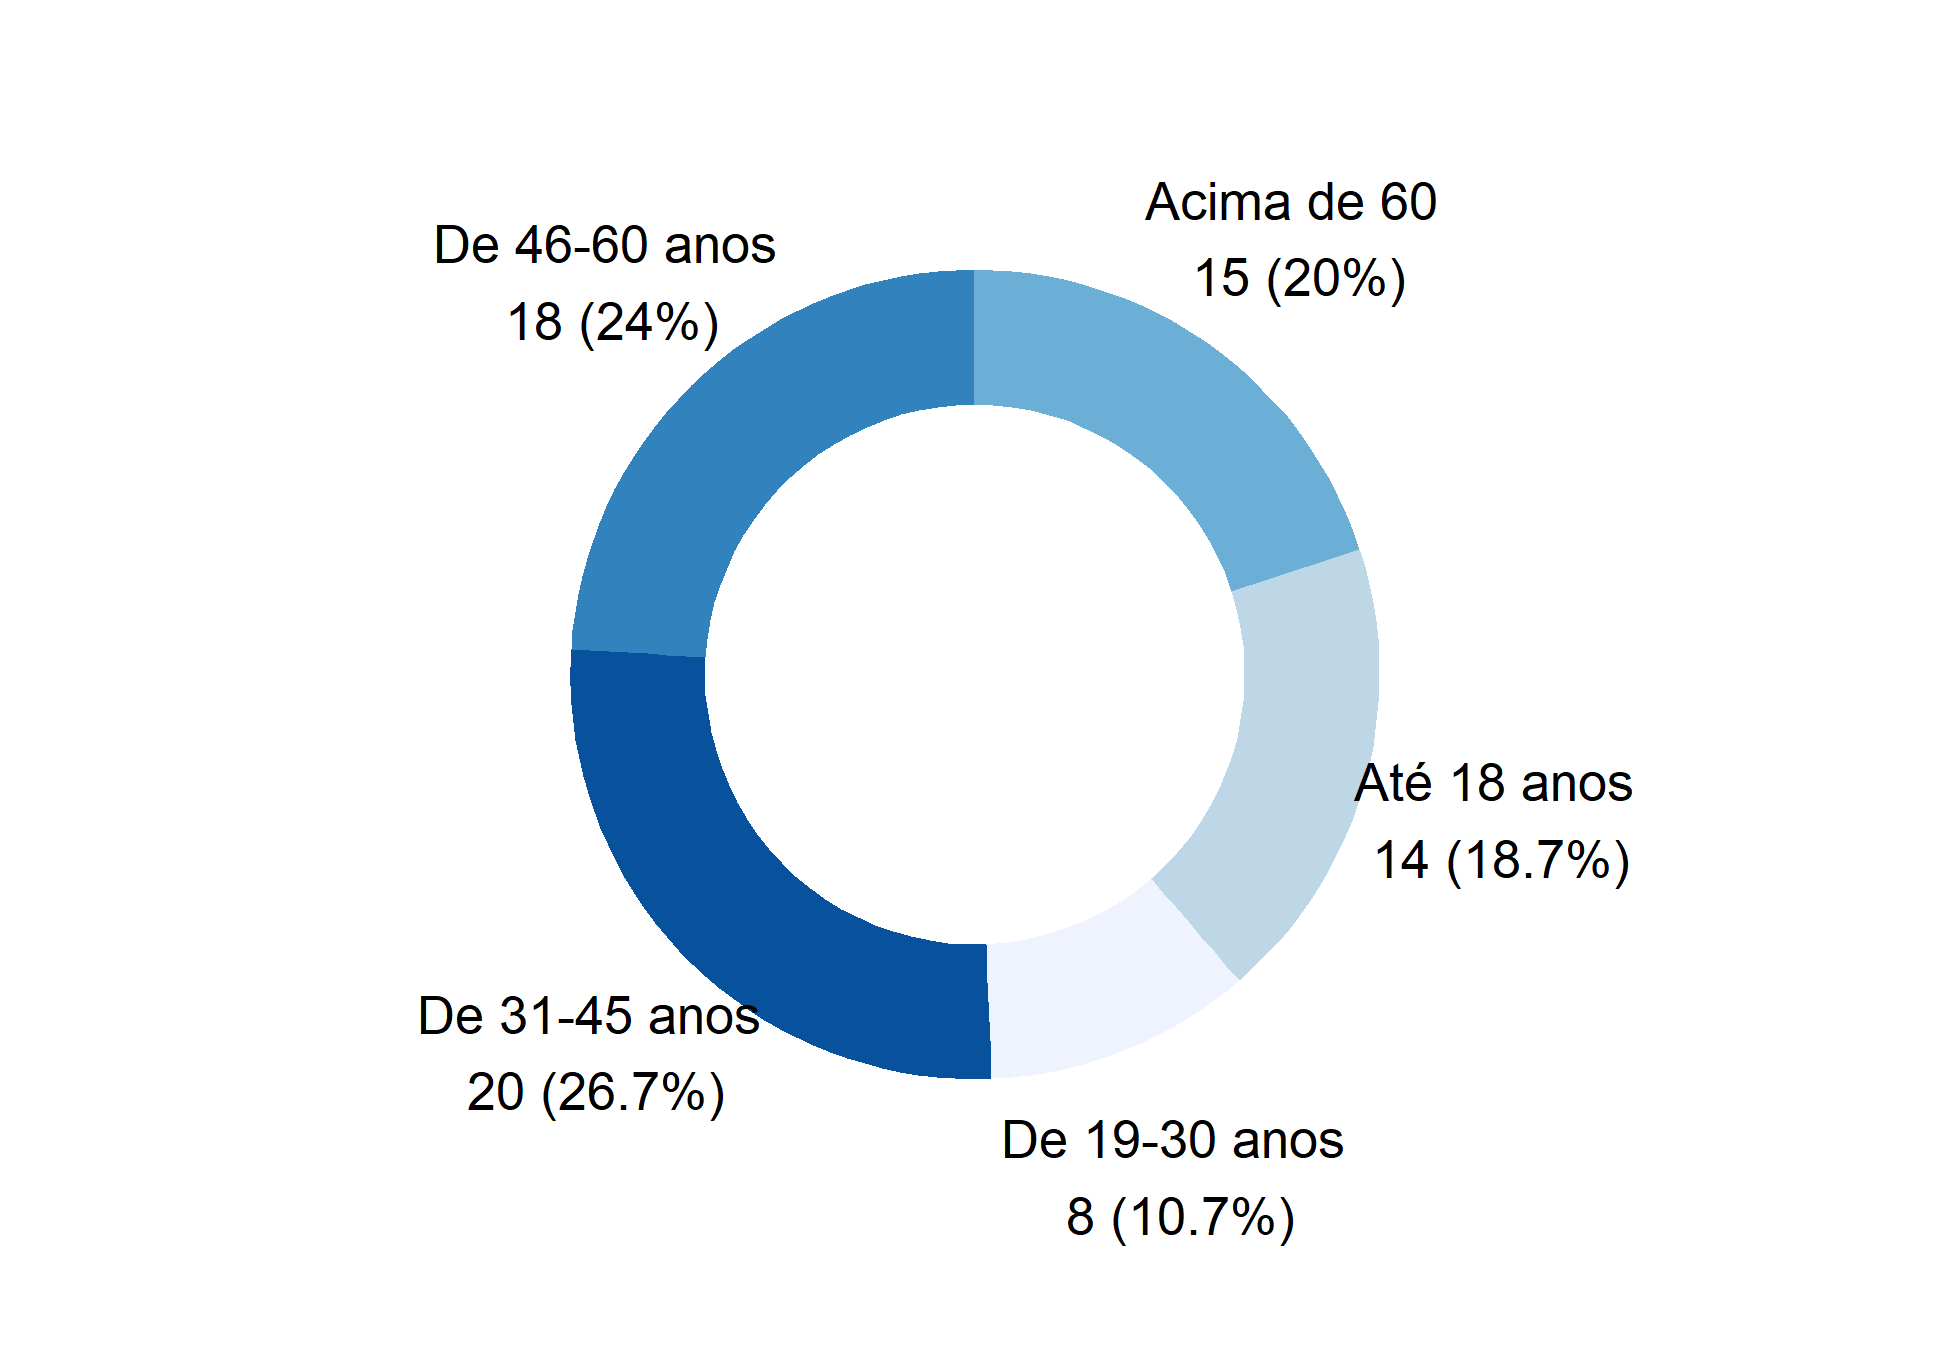
\includegraphics[width=0.7\textwidth]{Imagens/pele_faixa_etaria.png}
\end{figure}

\begin{table}[H]

\caption{\label{tab:unnamed-chunk-29}Tipo de Lesão de Pele}
\centering
\resizebox{\linewidth}{!}{
\begin{tabular}[t]{lrrrrrrrrrrrr}
\toprule
 & jan & fev & mar & abr & mai & jun & jul & ago & set & out & nov & Total\\
\midrule
Por adesivo & 2 & 3 & 9 & 5 & 2 & 8 & 4 & 4 & 6 & 7 & 2 & 52\\
Por queimaduras (exceto por bisturi elétrico) & 0 & 0 & 1 & 1 & 0 & 0 & 0 & 0 & 0 & 0 & 0 & 2\\
Por umidade & 4 & 2 & 3 & 0 & 0 & 0 & 2 & 1 & 0 & 2 & 0 & 14\\
\midrule
\textbf{Total} & \textbf{6} & \textbf{5} & \textbf{13} & \textbf{6} & \textbf{2} & \textbf{8} & \textbf{6} & \textbf{5} & \textbf{6} & \textbf{9} & \textbf{2} & \textbf{68}\\
\bottomrule
\end{tabular}}
\end{table}

\begin{table}[H]

\caption{\label{tab:unnamed-chunk-30}Comprometimento tissular da lesão por adesivo}
\centering
\begin{tabular}[t]{lr}
\toprule
Tipo de Adesivo & Total\\
\midrule
\midrule
\textbf{Total} & \textbf{0}\\
\bottomrule
\end{tabular}
\end{table}

\begin{table}[H]

\caption{\label{tab:unnamed-chunk-31}Tipo de Lesão por Umidade}
\centering
\begin{tabular}[t]{lr}
\toprule
Tipo & Total\\
\midrule
\midrule
\textbf{Total} & \textbf{0}\\
\bottomrule
\end{tabular}
\end{table}

\begin{table}[H]

\caption{\label{tab:unnamed-chunk-32}Comprometimento tissular da lesão por umidade}
\centering
\begin{tabular}[t]{lr}
\toprule
Manifestação cutânea & Total\\
\midrule
\midrule
\textbf{Total} & \textbf{0}\\
\bottomrule
\end{tabular}
\end{table}

\begin{table}[H]

\caption{\label{tab:unnamed-chunk-33}Localização da lesão por umidade}
\centering
\begin{tabular}[t]{lr}
\toprule
Localização da lesão & Total\\
\midrule
\midrule
\textbf{Total} & \textbf{0}\\
\bottomrule
\end{tabular}
\end{table}

\subsubsection{Medicamento}

\begin{table}[H]

\caption{\label{tab:unnamed-chunk-34}Classificação das notificações em medicamentos}
\centering
\resizebox{\linewidth}{!}{
\begin{tabular}[t]{lrrrrrrrrrrrr}
\toprule
 & jan & fev & mar & abr & mai & jun & jul & ago & set & out & nov & Total\\
\midrule
Evento Adverso & 3 & 3 & 1 & 5 & 4 & 4 & 5 & 5 & 13 & 5 & 3 & 51\\
Incidente sem dano & 11 & 24 & 16 & 8 & 19 & 22 & 10 & 18 & 11 & 14 & 13 & 166\\
Quase um erro (Near Miss) & 59 & 71 & 78 & 55 & 39 & 51 & 55 & 53 & 41 & 66 & 42 & 610\\
Sem classificacao & 0 & 0 & 1 & 0 & 0 & 0 & 0 & 0 & 0 & 0 & 0 & 1\\
\midrule
\textbf{Total} & \textbf{73} & \textbf{98} & \textbf{96} & \textbf{68} & \textbf{62} & \textbf{77} & \textbf{70} & \textbf{76} & \textbf{65} & \textbf{85} & \textbf{58} & \textbf{828}\\
\bottomrule
\end{tabular}}
\end{table}

\begin{table}[H]

\caption{\label{tab:unnamed-chunk-35}Notificações no processo de prescrição de medicamentos}
\centering
\begin{tabular}[t]{lr}
\toprule
Prescrição & Total\\
\midrule
Outros & 66\\
Dose incorreta & 62\\
Duplicidade de medicamento & 31\\
Falta de medicamento & 25\\
Frequência incorreta & 17\\
\addlinespace
Falta de frequência & 8\\
Medicamento incorreto & 8\\
Tempo de infusão incorreto & 8\\
Falta do tempo de infusão & 7\\
Uso de expressões vagas (SN, uso contínuo, a critério médico) & 6\\
\addlinespace
Falta de dose & 4\\
Forma farmacêutica ou apresentação incorreta & 4\\
Via de administração incorreta & 4\\
Medicamento contra-indicado & 3\\
Diluente/volume de diluente incorreto & 2\\
\addlinespace
Falta de horário & 2\\
Paciente incorreto & 2\\
Falta da apresentação farmacêutica & 1\\
Horário incorreto & 1\\
\midrule
\textbf{Total} & \textbf{261}\\
\bottomrule
\end{tabular}
\end{table}

\begin{table}[H]

\caption{\label{tab:unnamed-chunk-36}Notificações no processo de dispensação de medicamentos}
\centering
\begin{tabular}[t]{lr}
\toprule
Dispensação & Total\\
\midrule
Dose incorreta & 123\\
Falta de medicamento & 107\\
Medicamento incorreto & 49\\
Outros & 40\\
Medicamento com identificação incorreta/ausente & 25\\
\addlinespace
Horário incorreto & 12\\
Forma farmacêutica/apresentação incorreta & 5\\
Frequência incorreta & 5\\
Paciente incorreto & 5\\
Dispensado e não encontrado & 3\\
\addlinespace
Via de administração incorreta & 3\\
Diluente/volume de diluente incorreto & 1\\
\midrule
\textbf{Total} & \textbf{378}\\
\bottomrule
\end{tabular}
\end{table}

\begin{table}[H]

\caption{\label{tab:unnamed-chunk-37}Notificações no processo de preparo de medicamentos}
\centering
\begin{tabular}[t]{lr}
\toprule
Dispensação & Total\\
\midrule
Outros & 13\\
Aprazamento incorreto & 4\\
Diluente/volume de diluente incorreto & 3\\
Dose incorreta & 2\\
Medicamento incorreto & 1\\
\midrule
\addlinespace
\textbf{Total} & \textbf{23}\\
\bottomrule
\end{tabular}
\end{table}

\begin{table}[H]

\caption{\label{tab:unnamed-chunk-38}Notificação no processo de administração de medicamentos}
\centering
\begin{tabular}[t]{lr}
\toprule
Administração & Total\\
\midrule
Outros & 37\\
Medicamento não administrado (omissão) & 25\\
Horário incorreto & 21\\
Ausência de registro/checagem & 20\\
Velocidade/Tempo de infusão incorreto & 12\\
\addlinespace
Dose incorreta & 11\\
Medicamento incorreto & 11\\
Frequência incorreta & 8\\
Infiltração & 8\\
Paciente incorreto & 8\\
\addlinespace
Extravasamento & 7\\
Forma farmacêutica ou apresentação incorreta & 1\\
Medicamento fora de validade & 1\\
Via de administração incorreta & 1\\
\midrule
\textbf{Total} & \textbf{171}\\
\bottomrule
\end{tabular}
\end{table}

\subsection{Procedimento Cirúrgico}

\begin{figure}[H]
\caption{Distribuição do gênero nas notificações em Procedimento Cirúrgico.}
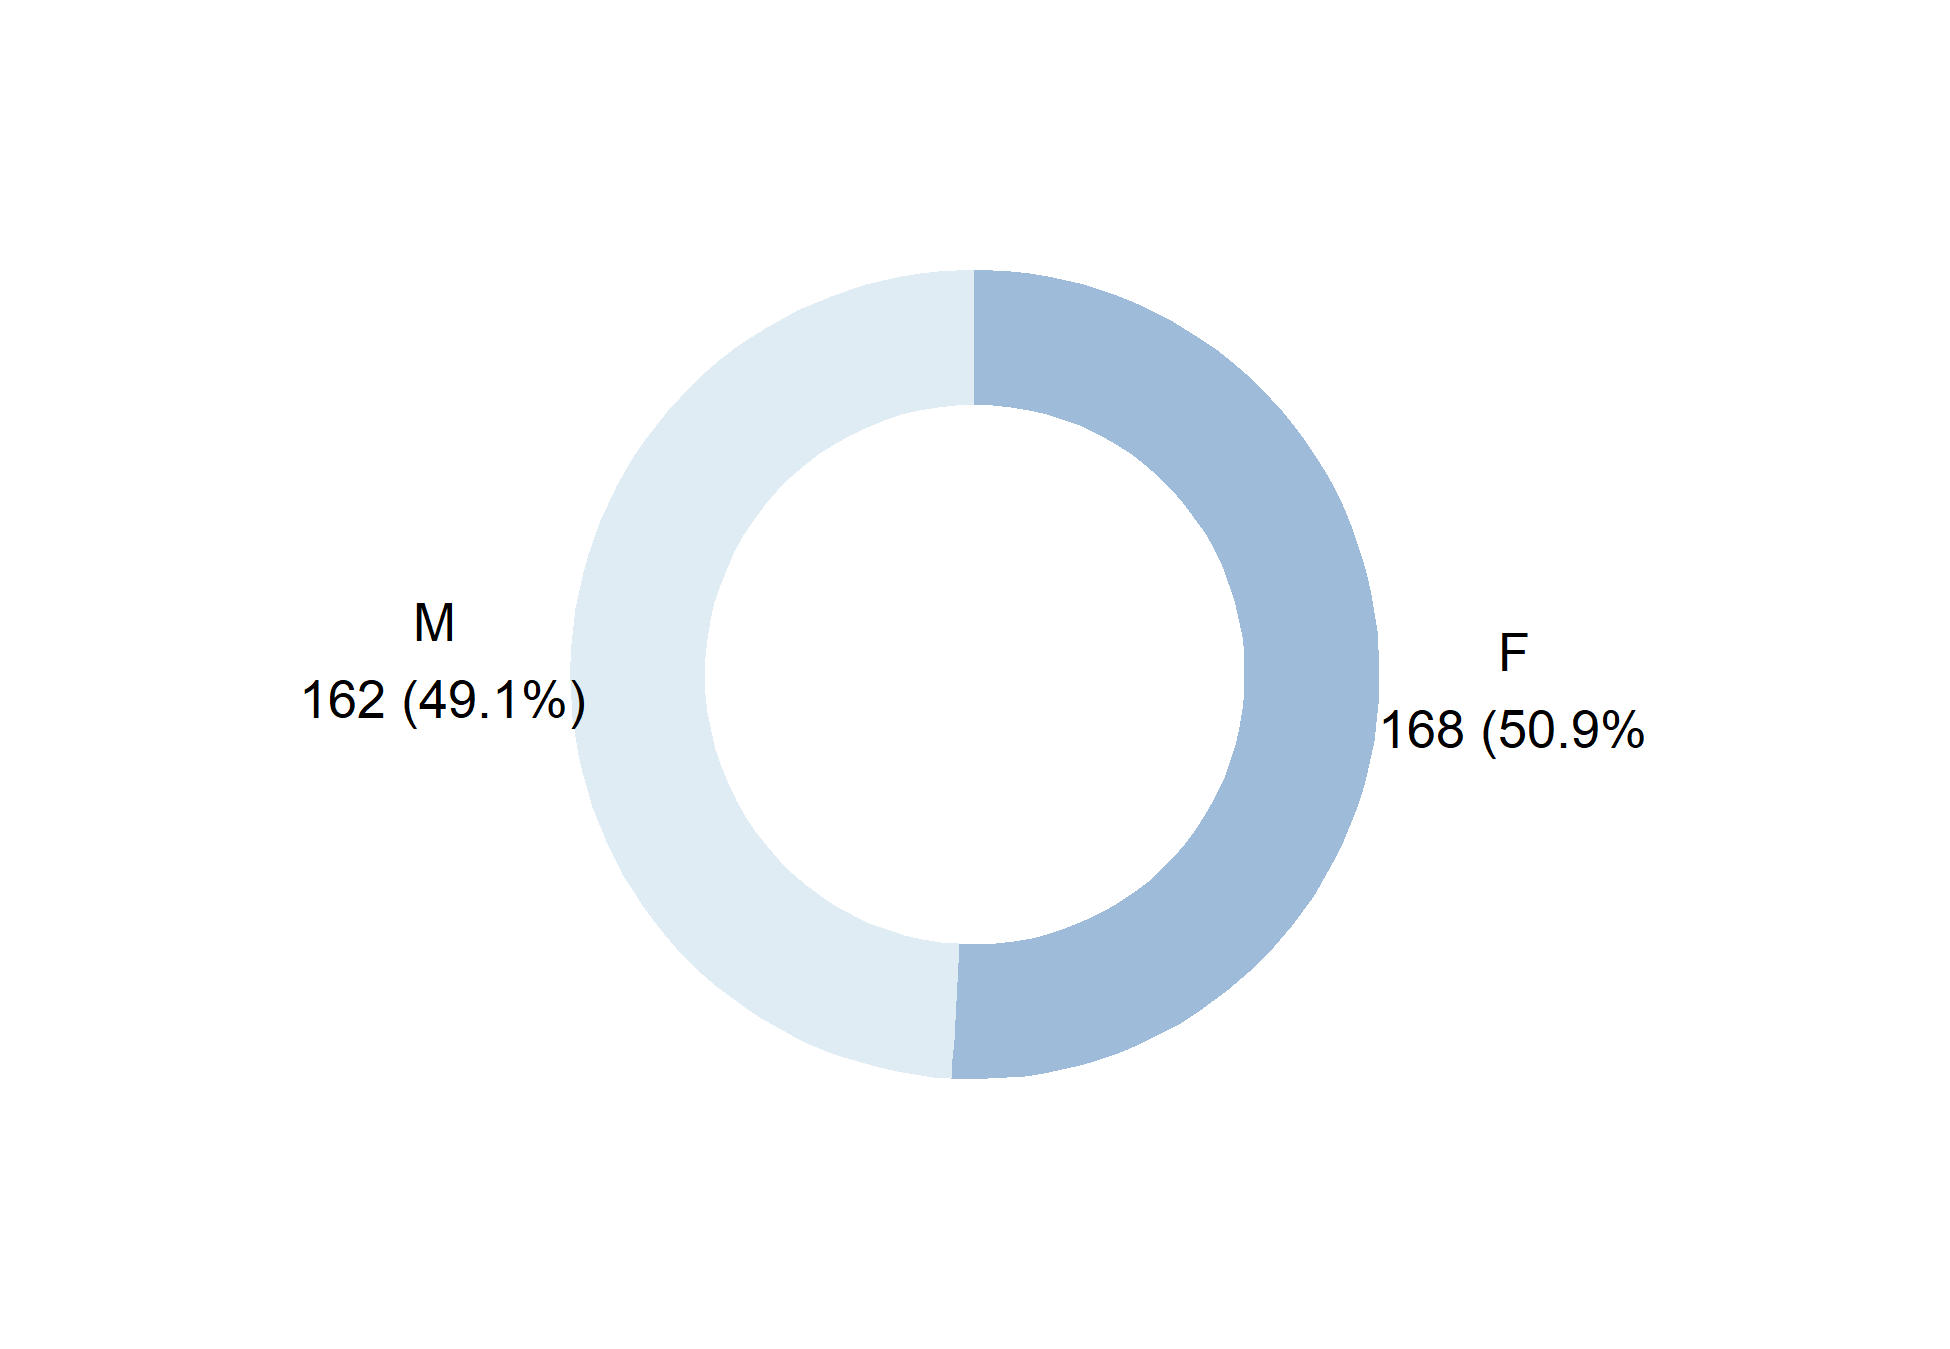
\includegraphics[width=0.7\textwidth]{Imagens/cirurg_SEXO.png}
\end{figure}

\begin{table}[H]

\caption{\label{tab:unnamed-chunk-40}Notificação de acordo com as fases do Procedimento Cirúrgico}
\centering
\resizebox{\linewidth}{!}{
\begin{tabular}[t]{lrrrrrrrrrrrr}
\toprule
 & jan & fev & mar & abr & mai & jun & jul & ago & set & out & nov & Total\\
\midrule
Intra-operatória & 1 & 2 & 0 & 0 & 1 & 1 & 0 & 1 & 1 & 0 & 0 & 7\\
Pós-operatória & 14 & 25 & 35 & 11 & 22 & 24 & 21 & 27 & 17 & 46 & 15 & 257\\
Pré-operatória & 2 & 1 & 1 & 1 & 3 & 2 & 1 & 0 & 0 & 1 & 0 & 12\\
Solicitação & 4 & 9 & 1 & 3 & 2 & 1 & 0 & 0 & 4 & 2 & 3 & 29\\
\midrule
\textbf{Total} & \textbf{21} & \textbf{37} & \textbf{37} & \textbf{15} & \textbf{28} & \textbf{28} & \textbf{22} & \textbf{28} & \textbf{22} & \textbf{49} & \textbf{18} & \textbf{305}\\
\bottomrule
\end{tabular}}
\end{table}

\begin{table}[H]

\caption{\label{tab:unnamed-chunk-41}Incidentes notificados da fase pós-operatória}
\centering
\begin{tabular}[t]{lr}
\toprule
Pós-operatória & Total\\
\midrule
Deiscência & 236\\
Não se aplica & 14\\
Maceração da ferida operatória & 13\\
Sofrimento da ferida operatória & 12\\
Hemorragia & 1\\
\midrule
\addlinespace
\textbf{Total} & \textbf{276}\\
\bottomrule
\end{tabular}
\end{table}

\begin{table}[H]

\caption{\label{tab:unnamed-chunk-42}Grau de dano das notificações da fase pós-operatória}
\centering
\begin{tabular}[t]{lr}
\toprule
Grau do Dano & Total\\
\midrule
Leve & 207\\
Moderado & 77\\
\midrule
\textbf{Total} & \textbf{284}\\
\bottomrule
\end{tabular}
\end{table}

\subsection{Dados Gerais de Notificação}

\begin{figure}[H]
\caption{Near miss notificados.}
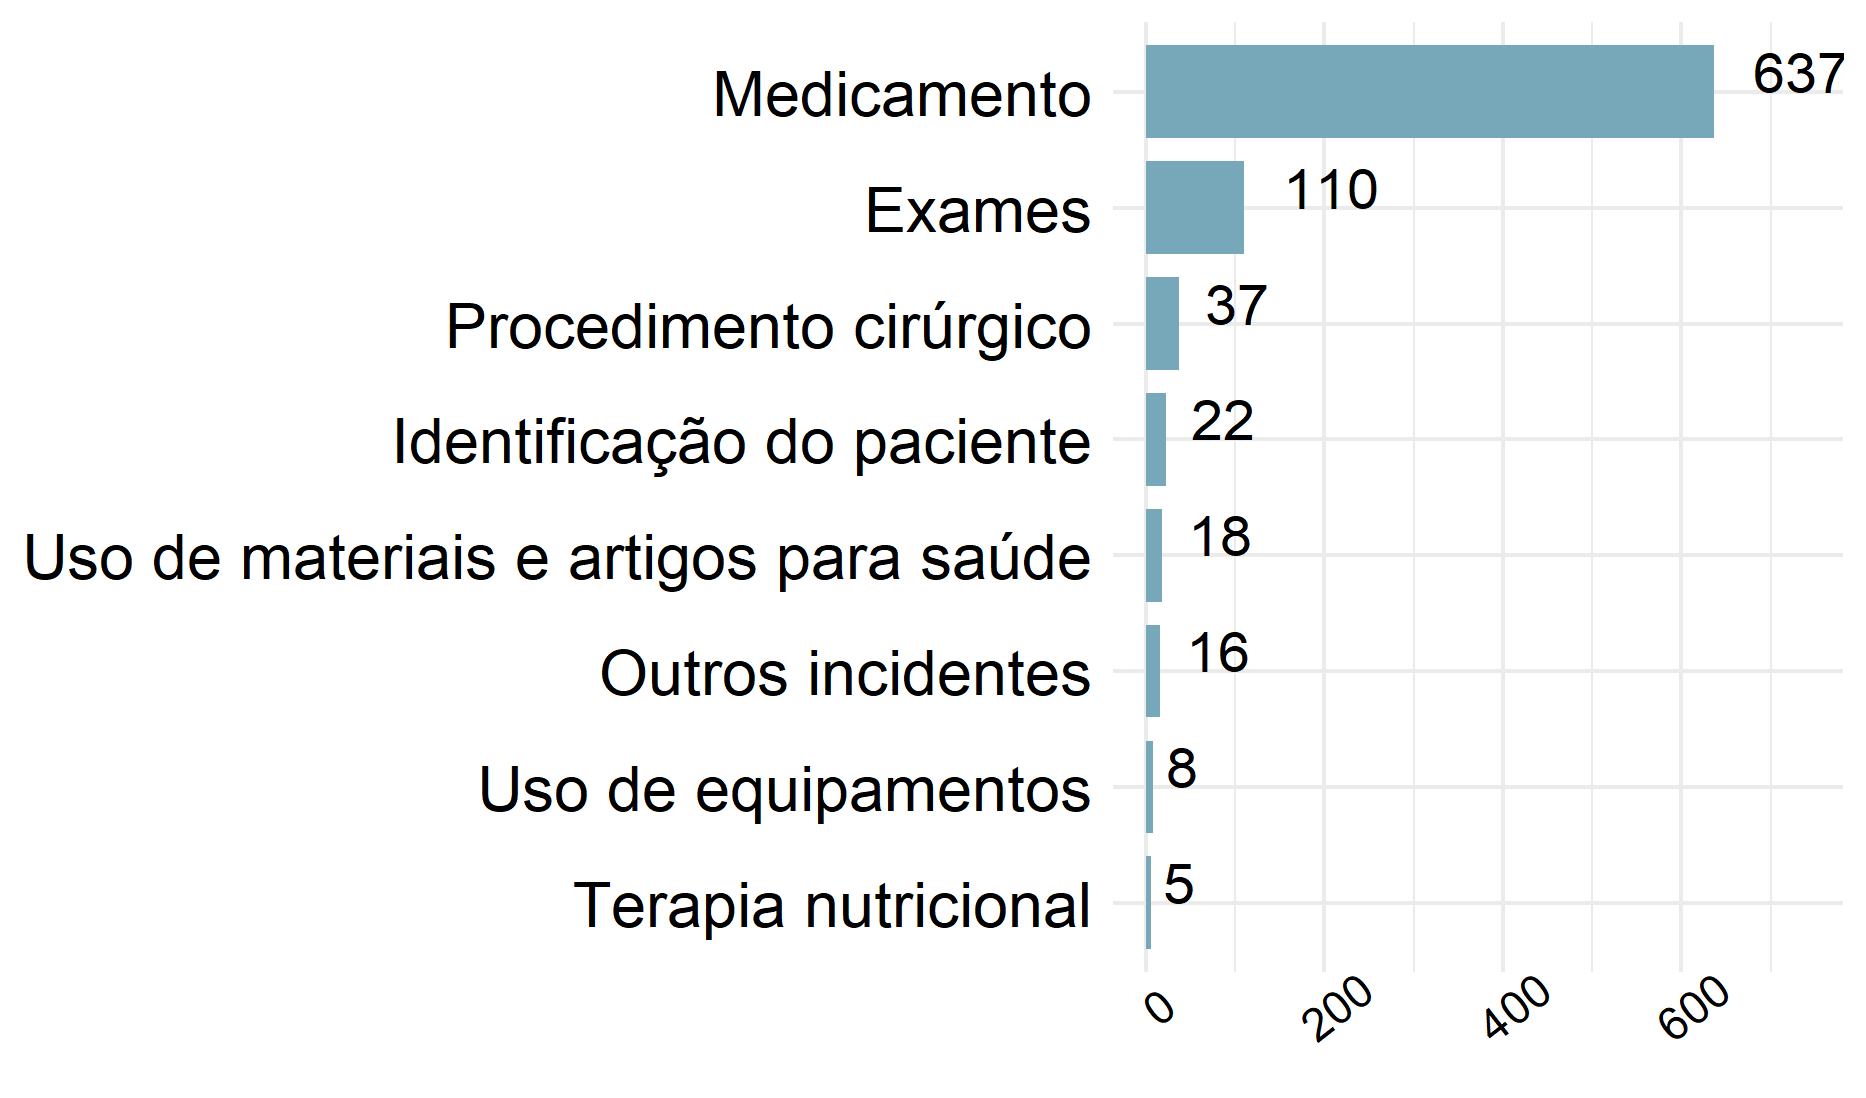
\includegraphics[width=0.7\textwidth]{Imagens/barra_erro.png}
\end{figure}

\begin{figure}[H]
\caption{Incidentes sem dano notificados.}
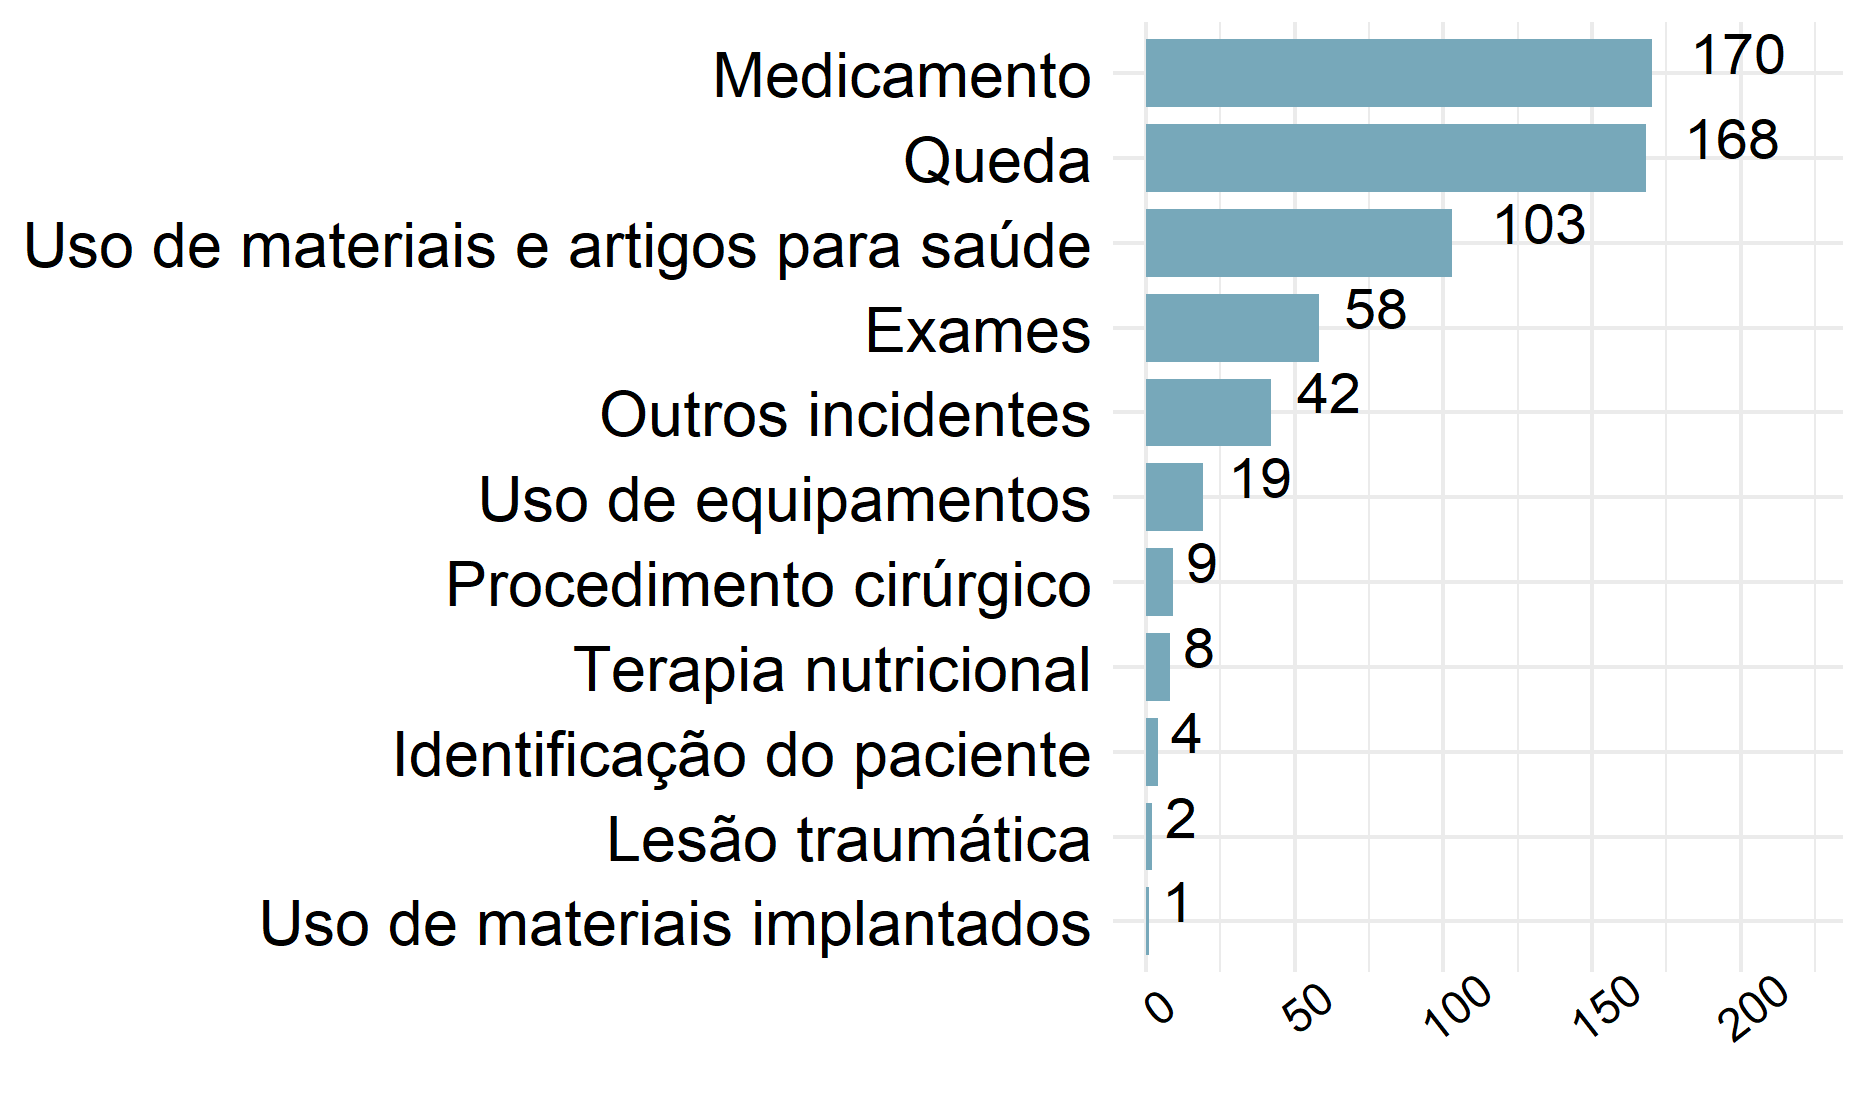
\includegraphics[width=0.7\textwidth]{Imagens/barra_incidente.png}
\end{figure}

\begin{figure}[H]
\caption{Eventos Adversos Notificados.}
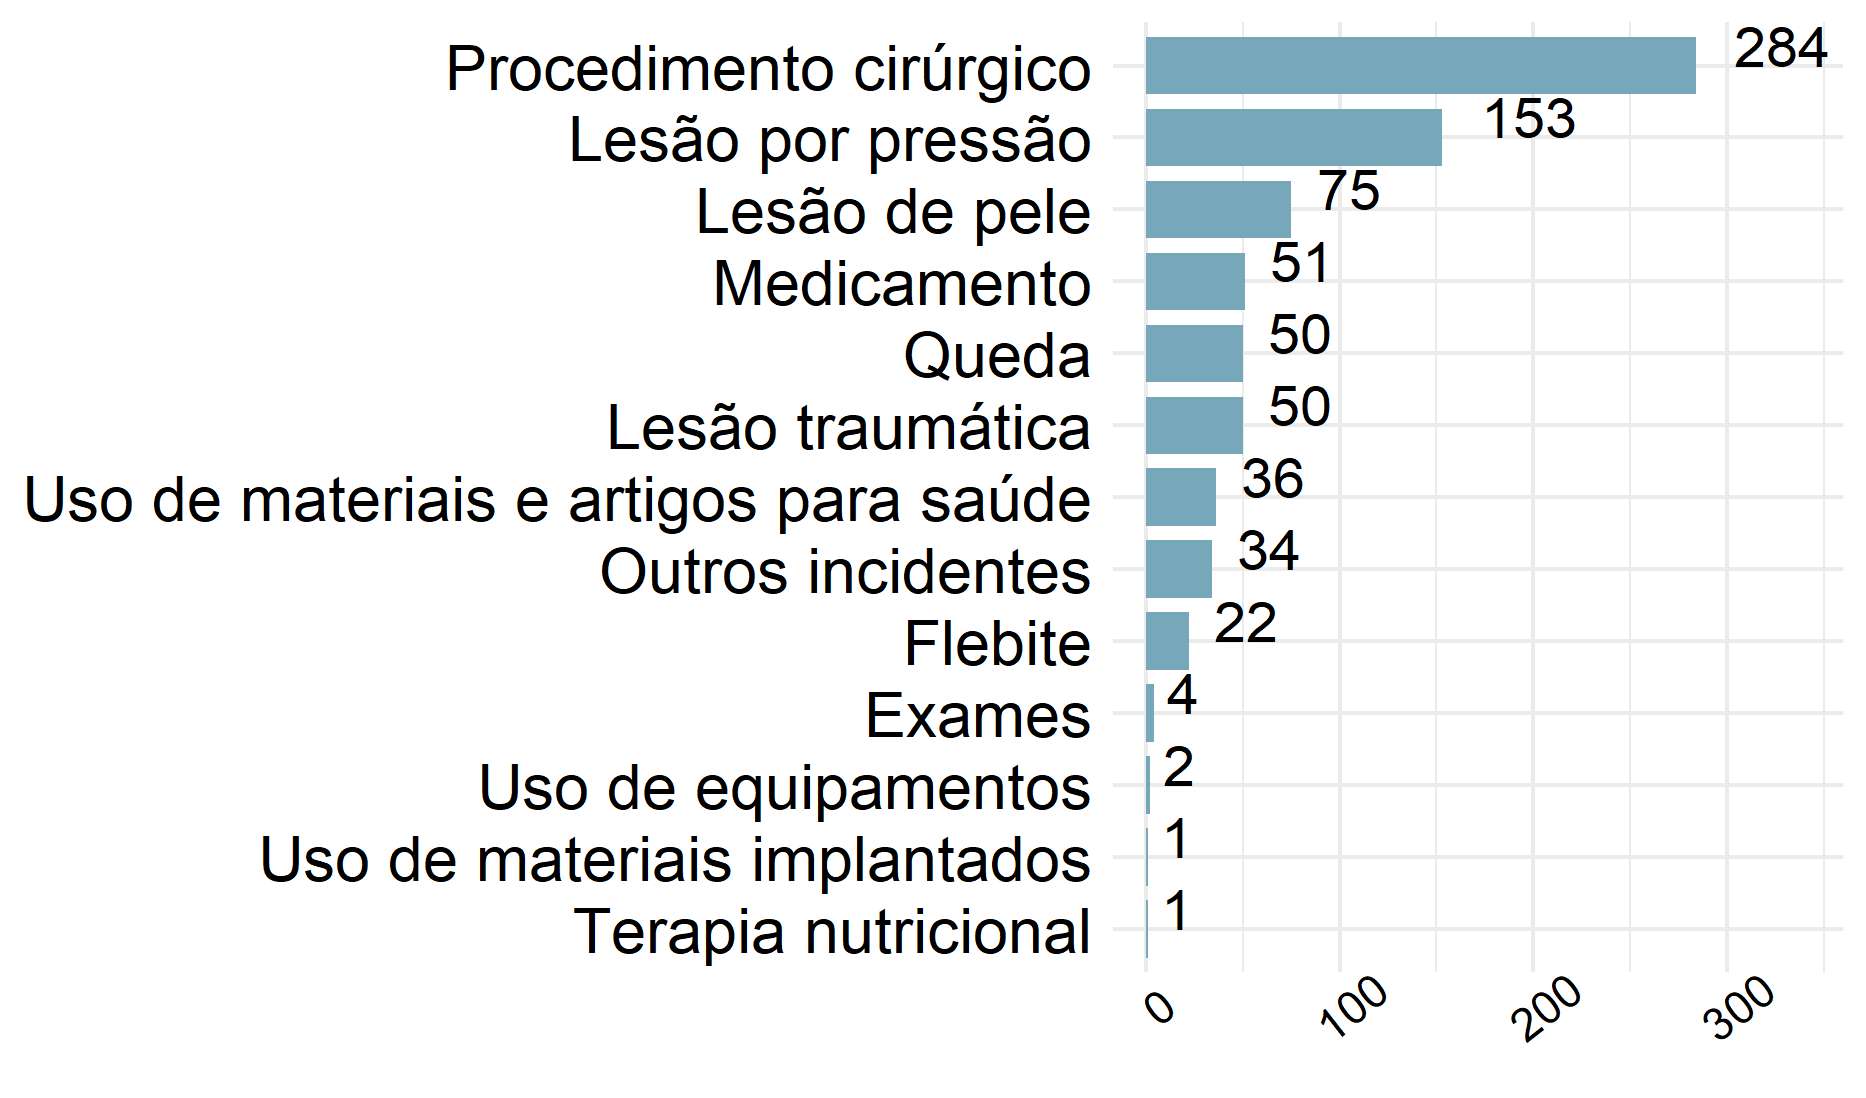
\includegraphics[width=0.7\textwidth]{Imagens/barra_evento.png}
\end{figure}

\end{document}
